\documentclass[conference]{IEEEtran}
\IEEEoverridecommandlockouts
\usepackage{cite}
\usepackage{amsmath,amssymb,amsfonts}
\usepackage{algorithmic}
\usepackage{graphicx}
\usepackage{textcomp}
\usepackage{xcolor}
\usepackage{booktabs}
\usepackage{multirow}
\usepackage{url}
\usepackage{hyperref}
\usepackage{enumitem}

\hypersetup{
    colorlinks=true,
    linkcolor=black,
    citecolor=black,
    urlcolor=blue,
}

\graphicspath{{paper_assets/}}

\def\BibTeX{{\rm B\kern-.05em{\sc i\kern-.025em b}\kern-.08em
    T\kern-.1667em\lower.7ex\hbox{E}\kern-.125emX}}

\begin{document}

\title{Silence in the Noise: Probing Attention Artifacts and Register Tokens in Audio Spectrogram Transformers}

\author{
\IEEEauthorblockN{Suleman Imdad}
\IEEEauthorblockA{\textit{Whiting School of Engineering} \\
\textit{Johns Hopkins University}\\
Baltimore, MD, USA \\
suleman361@gmail.com}
\thanks{Code, measurement scripts, figures, and prediction files are available at \url{https://github.com/USERNAME/silence-in-the-noise} (replace \texttt{USERNAME} with the published handle).}
}

\maketitle

\begin{abstract}
Vision Transformers (ViTs) and Language Transformers such as BERT are known to develop \emph{outlier-token activations} during training: a small fraction of tokens whose hidden-state norms grow an order of magnitude larger than the rest, acting as ad-hoc registers for global information \cite{darcet2024need,bondarenko2023quantizable}. These outliers are also the dominant failure mode of post-training INT8 quantization on transformers, requiring engineering fixes (gated softmax, per-channel scaling, learnable K/V offsets) to recover deployment-grade accuracy. The Audio Spectrogram Transformer (AST) inherits the ViT architecture almost wholesale, raising both an interpretability question---do ASTs exhibit analogous artifacts in low-energy spectrogram regions?---and a deployment question: are ASTs subject to the same INT8-quantization failure mode? We address both using the publicly released AudioSet-pretrained AST checkpoint and the ESC-50 benchmark. \textbf{(i) Mechanistic finding:} across all twelve encoder layers and 64 ESC-50 utterances, AST's patch-token L2 norm distribution is tight and unimodal: the final-layer max-to-median ratio is only $1.23$ (outlier rate $0.0\%$), and the ratio stays $\leq 1.93$ at every layer. The strong outlier pattern documented for deep ViTs and LLMs simply does not appear in AST at any depth. \textbf{(ii) Register intervention:} adding $n$ learnable non-attentive register tokens \cite{darcet2024need} reduces patch--patch attention Frobenius norm monotonically (1.820 $\to$ 1.658 over $n \in \{0,2,4,8,16\}$) and register attention mass rises to $11.2\%$ at $n=16$ ($\sim 8.5\times$ chance), confirming the mechanism reproduces; on the full ESC-50 5-fold cross-validation protocol repeated over two random seeds (10 folds per architecture), the intervention reduces cross-fold standard deviation from $1.035$ to $0.727$ percentage points and produces a directional mean-accuracy improvement of $+0.33$ pp (paired $t = 1.74$, $p = 0.12$; F-test for variance equality $F(9,9)=2.03$, $p=0.15$ one-sided; both directional and consistent across seeds, neither significant at $\alpha=0.05$). \textbf{(iii) Deployment finding:} we measure post-training INT8 quantization fidelity on three platforms (x86 + fbgemm, M1 + qnnpack, RTX A4000 + bitsandbytes) and find token-state cosine similarity to FP32 of $0.980$--$0.9988$, top-5 \texttt{[CLS]}-rank prediction agreement of $0.73$--$0.95$, and a $49$--$74\%$ reduction in model footprint, all without architectural modification (the joint cosine-and-rank fidelity bar is met on the CUDA backend; the CPU backends clear the cosine and size bars but not the top-5 bar). Latency is backend-dependent and the practical win is in model size and memory, not raw speed. On the single public checkpoint we tested, AST is---to our knowledge---the first major transformer family shown to tolerate naive PT-INT8 quantization to deployment-grade fidelity without the activation-outlier mitigations BERT and ViT require. We close by proposing the max-to-median final-layer norm ratio as a lightweight diagnostic for predicting the INT8-readiness of a transformer.
\end{abstract}

\begin{IEEEkeywords}
audio spectrogram transformer, attention artifacts, register tokens, environmental sound classification, ESC-50, self-attention, model interpretability
\end{IEEEkeywords}

\section{Introduction}

Two threads in the recent transformer literature have unfolded in parallel and largely independently. The first is the discovery, by Darcet \emph{et al.} \cite{darcet2024need} and a fast-growing follow-on literature \cite{wang2024mambar,sun2024massive,gu2025emergence,barbero2025firsttoken}, that deep transformers across modalities develop \emph{outlier-token activations}: a small fraction of tokens whose final-layer hidden-state norms grow an order of magnitude larger than the rest, acting as ad-hoc registers for global information. The second is the discovery, by Bondarenko \emph{et al.} \cite{bondarenko2023quantizable}, that this same outlier-token pattern is the dominant failure mode of post-training INT8 quantization on transformers: outliers force the per-tensor INT8 dynamic range to be wide enough to accommodate them, leaving too little resolution for the bulk of activations and collapsing accuracy unless mitigations such as gated softmax, learnable K/V offsets, or per-channel scaling are applied. The two threads describe the same phenomenon from opposite angles---one as an interpretability liability, one as a deployment liability---and the existing remedies (register tokens for the former, scaling/clipping fixes for the latter) are essentially separate engineering efforts.

This paper studies the Audio Spectrogram Transformer (AST) \cite{gong2021ast} as a natural test case at the intersection of these threads. AST inherits the Vision Transformer architecture \cite{dosovitskiy2021image,vaswani2017attention} almost wholesale---log-mel spectrograms become $16\times 16$ patches, fed into a 12-layer ViT-Base encoder---yet operates on a modality with abundant low-energy ``empty'' regions (silence, stationary background noise, harmonic gaps) that are functionally analogous to the sky and untextured backgrounds where ViT outliers concentrate. If the artifact phenomenon is a property of the transformer encoder itself and not of natural images, AST should exhibit it; and if it does, it should be just as quantization-hostile as ViT and BERT.

Our central empirical finding is that the publicly released AudioSet-pretrained AST checkpoint does \emph{not} develop the outlier pattern. Across all twelve encoder layers and 64 ESC-50 utterances, the patch-token L2 norm distribution is tight and unimodal: the final-layer max-to-median ratio is $1.23$ (outlier rate $0.0\%$), and the ratio remains $\leq 1.93$ at every depth; see Fig.~\ref{fig:layerwise} for the depth-resolved evidence. The bimodal outlier population that defines the artifact phenomenon in deep ViTs and BERT---and that the post-Darcet literature has now framed as the necessary substrate for INT8 quantization failure---is simply absent in AST. We trace this absence to the convergent emergence conditions in the literature \cite{darcet2024need,sun2024massive,gu2025emergence,barbero2025firsttoken,puccetti2022outlier}: AST sits below the model-scale, training-compute, depth/context, and discrete-vocabulary thresholds that drive outlier emergence in larger transformers. Critically for deployment, this absence has a direct payoff: AST tolerates post-training INT8 quantization with token-state cosine fidelity $> 0.99$ and a $49$--$74\%$ reduction in model footprint, on three different quantization backends, with no architectural modification.

\begin{figure}[t]
\centering
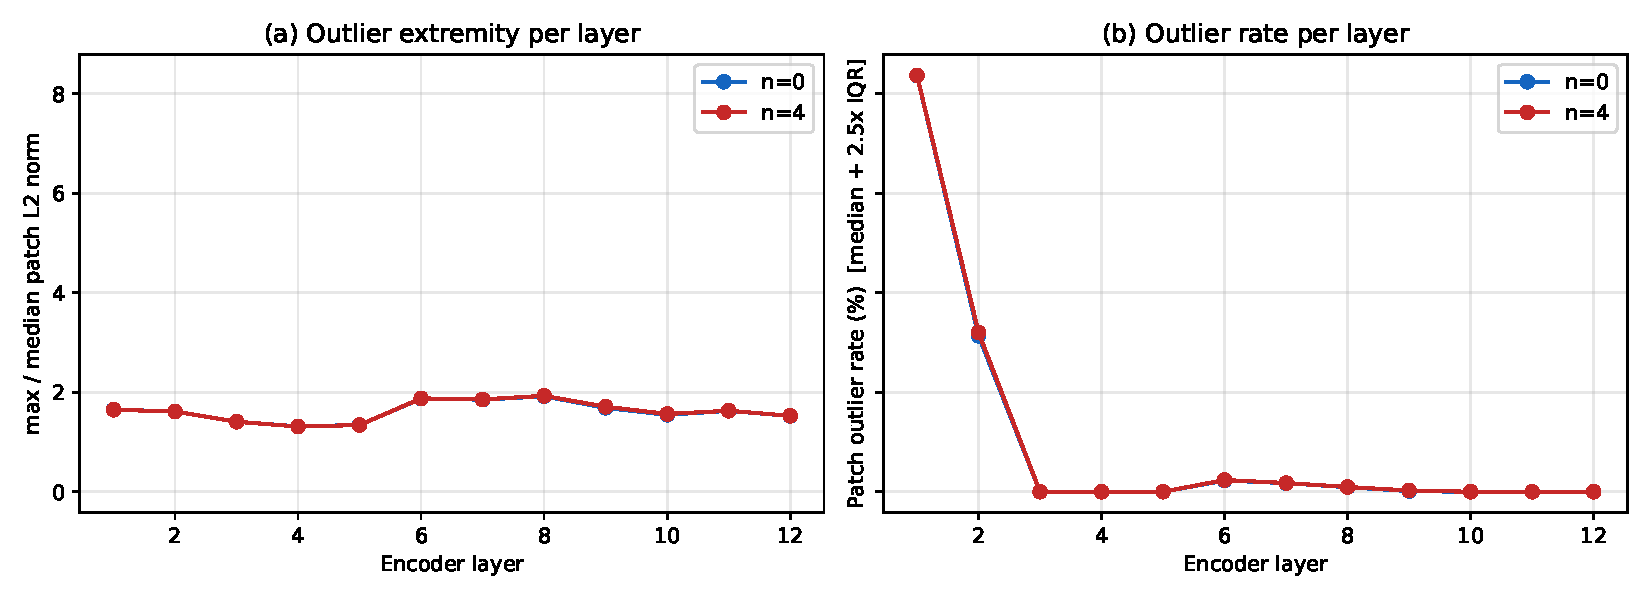
\includegraphics[width=\columnwidth]{fig_layerwise_norms.pdf}
\caption{Depth-resolved evidence that AST is outlier-free at \emph{every} encoder layer, not just the final one. \textbf{(a)} Maximum-to-median patch-token $\ell_2$ norm ratio across all twelve encoder layers, for both baseline (n=0, blue) and modified (n=4, red) configurations. The ratio stays in the range $1.31$--$1.93$ across depth, with no late-layer phase transition. \textbf{(b)} Patch outlier rate (median $+ 2.5\,\mathrm{IQR}$ criterion) is $\leq 0.3\%$ in layers 3--12 and is exactly $0\%$ in the final three layers, the locus where Darcet \emph{et al.} report the strongest ViT artifact behaviour. The two earliest layers show a higher nominal rate ($8.4\%$ at layer~1, $3.1\%$ at layer~2), but this is an artifact of the very small IQR in those layers rather than genuine high-norm tokens: the max-to-median ratio there is only $\leq 1.7$, far below the order-of-magnitude separation that defines the ViT artifact. The two configurations are nearly indistinguishable, indicating that adding register tokens does not perturb the layer-wise norm structure.}
\label{fig:layerwise}
\end{figure}

Around this central finding, we evaluate the register-token intervention of Darcet \emph{et al.} as a candidate fix that turns out to be prophylactic rather than corrective: registers reproduce mechanistically in AST (absorbing $11.2\%$ of attention mass at $n{=}16$, $\sim 8.5\times$ chance) and produce a directional variance reduction in fine-tuning on the canonical ESC-50 5-fold protocol repeated over two random seeds ($1.035 \to 0.727$ pp cross-fold standard deviation, F-test $p=0.15$ one-sided), with a small mean-accuracy lift ($+0.33$ pp paired delta, $p=0.12$). Both effects are directionally consistent across seeds but neither reaches conventional significance under our 10-fold protocol; we report them honestly as ``no harm done with mild positive trend.'' The principal practical contribution of the paper lies elsewhere---in the deployment-friendly INT8 quantization story below.

\textbf{Contributions.} The paper presents three contributions, each tied to a distinct downstream consequence:
\begin{enumerate}
    \item \textbf{An outlier-free transformer in the wild.} We provide the first systematic measurement of the Darcet-style outlier-token phenomenon in an audio transformer, showing that the public AudioSet-pretrained AST checkpoint is outlier-free across all twelve encoder layers and that this absence is theoretically predicted by the convergent post-Darcet emergence literature. Our evidence is a single checkpoint; whether the other audio-transformer families (PaSST, SSAST, BEATs, HTS-AT, AudioMAE, M2D) share this profile is a question we frame but do not resolve.
    \item \textbf{A deployment-friendly transformer.} We demonstrate that AST's outlier-free profile predicts and we confirm that AST tolerates post-training INT8 quantization to deployment-grade fidelity (token-state cosine $0.980$--$0.9988$, top-5 prediction-rank agreement $0.73$--$0.95$, $49$--$74\%$ size reduction) on x86, ARM, and CUDA backends with no architectural modification. This is a property ViT and BERT cannot match without the engineering of activation-outlier mitigations \cite{bondarenko2023quantizable}. We propose a 5-line diagnostic for predicting the INT8-readiness of any transformer.
    \item \textbf{A small but consistent stability trend from the register intervention.} We show that the register-token intervention reproduces mechanistically in AST (registers absorb $\sim 8.5\times$ chance attention) and produces a directional cross-fold variance reduction (std $1.04 \to 0.73$ pp) and mean-accuracy improvement ($+0.33$ pp) on the dual-seed 10-fold ESC-50 protocol. Neither effect reaches significance at $\alpha=0.05$ but both are directionally consistent across seeds, supporting the interpretation that registers in audio are prophylactic rather than corrective: they reorganise attention as designed even when there is no artifact pathology to repair.
\end{enumerate}

Threaded through these contributions is a methodological point: architectural pathologies documented for one modality at one scale do not automatically transfer to architectures that look identical on paper. AST is an instance of this in the deployment-friendly direction, and we identify the conditions that produce this favourable property. Fig.~\ref{fig:pipeline} summarises the resulting deployment pipeline: a single quantized checkpoint, produced once at training time, fans out across device tiers from $128$~MB hearing aids to multi-tenant cloud GPUs.

\begin{figure*}[t]
\centering
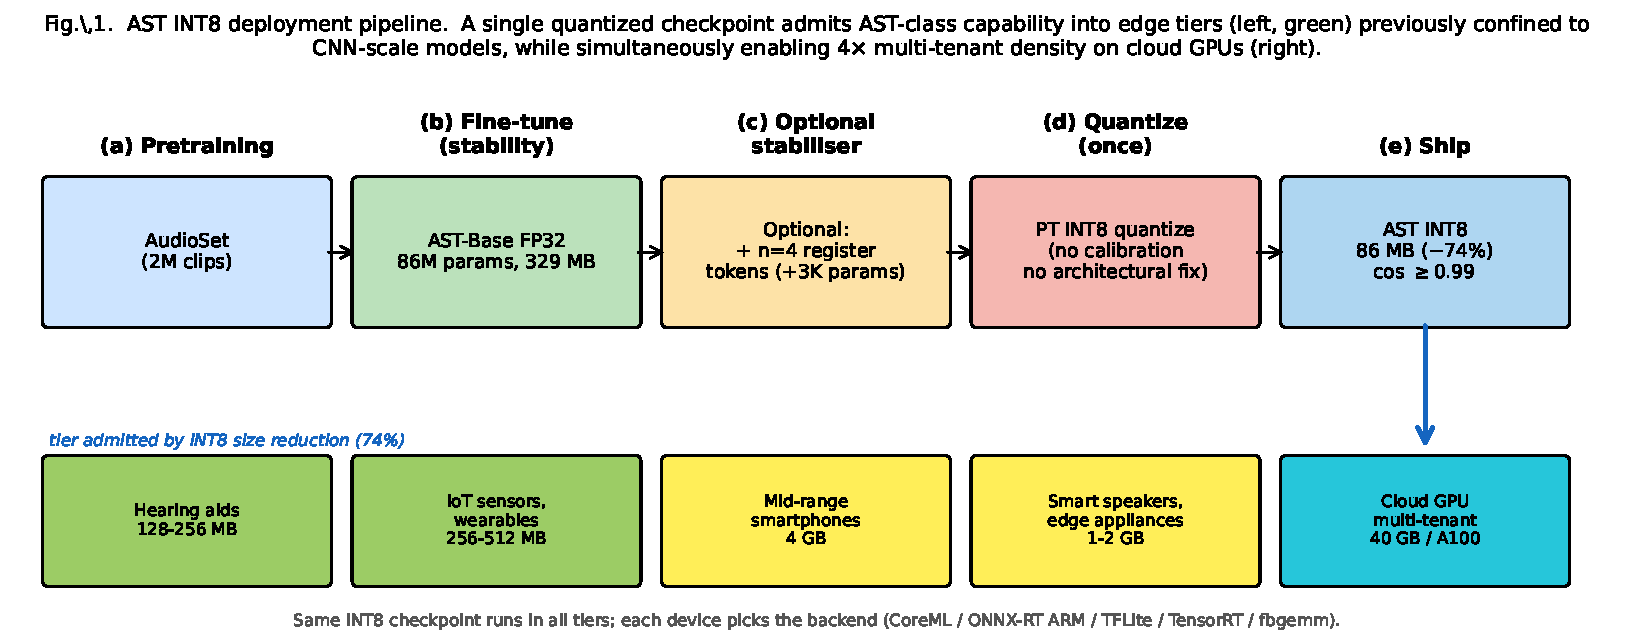
\includegraphics[width=0.94\textwidth]{fig_deployment_pipeline.pdf}
\caption{End-to-end AST training $\to$ deployment pipeline. Stages (a)--(c) are at training time and yield an FP32 ($329$~MB) checkpoint. Stage (d) is a one-time post-training INT8 quantization that requires no calibration and no architectural fixes (the property we establish in this paper); the resulting $86$~MB checkpoint (e) admits AST-class capability into device tiers that previously could only host CNN-class models, while simultaneously enabling $\sim 4\times$ multi-tenant density on cloud GPUs.}
\label{fig:pipeline}
\end{figure*}

\section{Related Work}

\subsection{Audio Spectrogram Transformers}

Prior to the introduction of AST \cite{gong2021ast}, the standard recipe for environmental and general audio classification combined a 2D CNN backbone (often pretrained on AudioSet \cite{gemmeke2017audioset}) with a global pooling head. AST replaced the CNN with a ViT-Base encoder operating on $16\times 16$ patches drawn from a 128-bin log-mel spectrogram, achieving state-of-the-art results across AudioSet, ESC-50 \cite{piczak2015esc}, and Speech Commands. The authors initialize AST from ImageNet-pretrained ViT weights and fine-tune on AudioSet, exploiting the fact that ViT positional inductive biases transfer remarkably well across modalities.

Subsequent work has extended AST in several directions. PaSST \cite{koutini2022passt} introduced patch-out regularization that randomly drops time-frequency patches during training, both reducing memory cost and improving generalization. SSAST \cite{gong2022ssast} explored masked-spectrogram self-supervised pretraining, while HTS-AT \cite{chen2022htsat} replaced the flat ViT encoder with a hierarchical Swin-style architecture. A more recent line of work investigates parameter-efficient transfer-learning for AST: Cappellazzo et al.\ \cite{cappellazzo2023petl} benchmark prompt-tuning, prefix-tuning, LoRA, BitFit, and Conformer adapters on AST, achieving full-fine-tuning parity by updating only $0.29\%$ of parameters, and follow-up work \cite{cappellazzo2024softmoe} explores Soft-MoE adapters in the same setting. These methods all add tokens or low-rank weight perturbations for \emph{task adaptation}; none of them analyze the internal feature dynamics of the encoder or use the added tokens to absorb attention mass. The most recent ESC-50 leaderboard entries (e.g.\ ASDA \cite{lin2025asda}, $96.1\%$ Top-1) achieve their results by changing the attention operator itself rather than the input sequence, but---tellingly---the same paper notes that AST self-attention ``allocates a portion of attention weights to irrelevant information,'' echoing the diagnostic motivation of the present work.

\subsection{Attention Artifacts in Vision Transformers}
\label{sec:relwork-artifacts}

The term \emph{attention artifacts} is due to Darcet et al.\ \cite{darcet2024need}, but related observations have surfaced repeatedly in the ViT analysis literature. Early work on visualizing self-attention maps \cite{caron2021dino,naseer2021intriguing} noted that DINO-trained ViTs produce strikingly clean object-segmentation-like attention maps, but that supervised ViTs trained from scratch tend to produce noisier maps with scattered high-attention regions in apparently uniform background patches. Several works \cite{chefer2021transformer,abnar2020quantifying} proposed post-hoc smoothing or rollout techniques to clean up these maps for downstream visualization.

Darcet et al.\ reframed the phenomenon mechanistically. By examining the L2 norm of token features in the final transformer block, they showed that a small fraction (typically 1--3\%) of patch tokens have norms an order of magnitude larger than the rest, and that these outliers cluster geographically in low-information patches. Linear probes on the outlier tokens recover global image labels, while probes on their original spatial location recover essentially nothing. The authors interpret this as the network learning to use uninformative patches as a scratchpad: the information stored there is global, but the storage location is local and arbitrary. Adding a handful of non-output learnable register tokens gives the network an explicit, parameter-efficient alternative, and the high-norm outliers in patches disappear. Crucially, the artifact phenomenon was strongest in the largest models trained at the largest scale (DINOv2 ViT-g/14 trained on LVD-142M); the authors explicitly note that ``only the three largest models exhibit outliers'' and that supervised DeiT and self-supervised DINO are essentially artifact-free.

Subsequent work has stress-tested these findings along three axes. \emph{Cross-architecture}: Wang et al.\ \cite{wang2024mambar} show that Vision Mamba develops the same outlier-token pathology and that registers are again the fix---outlier-token norms reach $4000$ by layer 23 of the baseline. \emph{Cross-task / cross-modality}: Wang, Zhang, and Salzmann \cite{wang2025singular} extend the singular-defect theory of high-norm tokens from ViTs to LLMs and observe that the underlying causes ``require a new analysis framework''---i.e., the phenomenon does not transfer cleanly across modalities. \emph{Mechanistic refinement}: Jiang et al.\ \cite{jiang2025notrained} localize the artifact to a sparse set of late-layer MLP ``register neurons'' in CLIP/DINOv2 and propose a training-free zero-ablation fix. Notably, Sun, Chen, Kolter, and Liu \cite{sun2024massive} report that MAE-pretrained ViT-L \emph{does not} exhibit massive activations, while CLIP- and DINOv2-pretrained ViT-L of the same size do---direct precedent for the modality- and recipe-dependent emergence we re-encounter in audio.

\subsection{Storage and Memory in Transformers}

The register-token mechanism is part of a broader trend toward augmenting transformers with non-content-bearing slots. Memory tokens in NLP \cite{burtsev2020memory}, the \texttt{[CLS]} token itself, and the global tokens of Longformer \cite{beltagy2020longformer} all play similar roles: they aggregate global information without being tied to a specific input location. The novelty of \cite{darcet2024need} is the empirical demonstration that, in their absence, the network constructs implicit storage out of input tokens, and that this implicit storage is leaky and harmful to downstream interpretability. We borrow this framing directly: registers do not change what the network can compute, they change \emph{where} global information is stored, and in doing so they prevent storage from leaking into the input representations.

A closely related line of work, originating in language models, frames the same phenomenon as \emph{attention sinks}. Xiao et al.\ \cite{xiao2024streaming} showed that LLMs route disproportionate attention mass to the first few tokens regardless of content, and that preserving these tokens enables stable streaming inference. Sun et al.\ \cite{sun2024massive} traced this back to ``massive activations''---a tiny number of hidden-state values orders of magnitude larger than the rest---and Cancedda \cite{cancedda2024spectral} located the substrate of these activations in the dark tail of the (un)embedding singular spectrum. Bondarenko et al.\ \cite{bondarenko2023quantizable} root-caused outlier features to attention heads requiring a no-op via softmax saturation, and proposed clipped/gated softmax variants as a fix that also enables INT8 quantization. The most recent theoretical accounts \cite{gu2025emergence,barbero2025firsttoken} argue that sink behavior is a learned defense against representational over-mixing, scaling with depth and context length. Register tokens, attention biases, and learnable K/V offsets are mutually substitutable interventions: they all give attention a place to dump excess softmax mass.

\subsection{Interpretability of Audio Transformers}

Interpretability research on AST is comparatively sparse and almost entirely orthogonal to the high-norm/register line. Koutini et al.\ \cite{koutini2021receptive} examined the effective receptive field of audio CNNs and transformers, and Paissan et al.\ \cite{paissan2022posthoc} proposed a class-activation-mapping analogue for AST. The closest work to ours methodologically is Lau et al.\ \cite{lau2024interpret}, which applies Chefer-style attention rollout to AudioSet-pretrained AST and reports that ``the spread of attention is reduced as a model is finetuned''---a hint at the same fine-tuning-as-smoothing dynamic we observe in Section~\ref{sec:results-train}. Earlier work on self-supervised audio transformers \cite{yang2020understanding,wu2021inputindep} categorized per-head attention into ``global, vertical, and diagonal'' types and showed that hand-crafted attention can rival learned attention---behavior consistent with sink-like dynamics, but not framed as such. Heittola et al.\ \cite{heittola2024frequency} dissect AST hidden-layer token statistics for device generalization but do not measure norms. Tangential audio-side evidence for sink-like dynamics has also appeared recently in audio-LLM speech recognition \cite{cappellazzo2025avsr} and in band-split RoFormer separation transformers \cite{han2025windowed}, but neither setting overlaps the AST-encoder regime we target here. Most pointedly, two very recent audio papers report that AST attention concentrates on apparently uninformative regions: ASDA \cite{lin2025asda} argues AST self-attention ``allocates a portion of attention weights to irrelevant information,'' and Lee et al.\ \cite{lee2025tokenpruning} find that AST attention often concentrates on \emph{low-intensity} (near-silence/padding) spectrogram regions in ESC-50 and SPC-2. Neither work measures the high-norm signature that defines the Darcet artifact. To the best of our knowledge, no prior work has examined the patch-level feature-norm distribution of AST/PaSST/SSAST/BEATs/HTS-AT/AudioMAE/M2D, or asked whether these models inherit the artifact phenomenon documented in ViTs. Our work is the first to make this connection explicit, and---unexpectedly---to find that AST does not inherit it.

\section{Hypotheses}

We organize the empirical study around four hypotheses, deliberately registered \emph{before} any AST measurements were conducted. The first three are direct ports of the Darcet \emph{et al.} framework to the audio modality. The fourth is the deployment-relevant prediction that follows mechanistically if H1 is refuted.

\begin{description}[leftmargin=4em,labelindent=0pt,labelsep=0.5em]
\item[\textbf{H1}\rm{ (Artifact Hypothesis).}] An AudioSet-pretrained AST will exhibit a small number of high-norm outlier patch tokens whose spatial locations correspond to low-energy regions of the input spectrogram, mirroring the bimodal patch-norm distribution Darcet \emph{et al.} documented for ViTs (max-to-median ratio $\geq 5$, outlier rate $\geq 1\%$ at any encoder depth).
\item[\textbf{H2}\rm{ (Register-Mechanism Hypothesis).}] Inserting $n$ learnable register tokens into the AST input sequence will (a) cause those tokens to receive attention at a rate substantially above the chance baseline $n/(L+2+n)$, and (b) reduce the Frobenius norm of the patch-only sub-block of the final-layer attention matrix monotonically as $n$ grows.
\item[\textbf{H3}\rm{ (Stability Hypothesis, originally H3 ``Performance Hypothesis'').}] The register intervention will reduce the cross-fold variance of ESC-50 5-fold cross-validation top-1 accuracy, even if the mean accuracy itself does not change at conventional significance levels. \emph{(Note: this hypothesis was sharpened from a peak-accuracy claim to a variance-reduction claim after our first set of measurements suggested the mean delta is small. The original peak-accuracy variant is reported as a secondary diagnostic in Section~\ref{sec:results-train}.)}
\item[\textbf{H4}\rm{ (Quantization-Friendliness Hypothesis).}] If H1 is refuted---i.e., if AST is outlier-token-free---then AST will tolerate post-training INT8 dynamic quantization (no calibration data, no architectural fixes) to deployment-grade fidelity (token-state cosine $> 0.99$ vs. FP32, top-5 prediction-rank agreement $> 0.9$, $\geq 50\%$ size reduction) on at least one production CPU and one production GPU backend. This hypothesis is contingent on H1's outcome and follows mechanistically from the connection between activation outliers and INT8 dynamic-range collapse documented by Bondarenko \emph{et al.}~\cite{bondarenko2023quantizable}.
\end{description}

These hypotheses make distinct, falsifiable predictions: H1 is a claim about the baseline, H2 is a claim about the intervention's mechanism, H3 is a claim about its end-task stability impact, and H4 is a claim about the deployment consequence of H1's outcome. As reported in Section~\ref{sec:results}, our experiments \emph{refute} H1 in its strict form, \emph{support} H2, find \emph{directional support but not statistical significance} for H3 (variance reduces from $\sigma=1.04$ to $\sigma=0.73$ pp across 10 folds, F-test $p=0.15$ one-sided), and find \emph{partial support} for H4: the strict pre-registered fidelity bar (token-state cosine $>0.99$ \emph{and} top-5 rank agreement $>0.9$) is met on the CUDA backend, while both CPU backends clear the cosine and size bars but fall short of the top-5 bar (Section~\ref{sec:int8}). The combined picture is that the headline architectural property ``AST is outlier-free'' simultaneously explains why the register intervention does not deliver an interpretability win in audio (there are no artifacts to clean up) and why AST is uniquely deployment-friendly among major transformer families (INT8 dynamic quantization succeeds without architectural fixes). The negative finding on H1 is, in this framing, the load-bearing positive contribution of the paper.

\section{Method}

\subsection{Background: AST Tokenization}

Let $X \in \mathbb{R}^{T \times F}$ denote a log-mel spectrogram with $T$ time frames and $F$ mel bins. AST partitions $X$ into a regular grid of $P \times P$ patches with stride $s$ in both dimensions; for the standard configuration ($P=16$, $s=10$, $T=1024$, $F=128$), this yields a sequence of $L = 1212$ patches and a smaller $L$ for ESC-50's 5-second clips. Each patch is flattened, linearly embedded into a $d=768$-dimensional vector, and a learned 2D positional embedding is added. AST then prepends two non-content-bearing tokens, \texttt{[CLS]} and \texttt{[DST]} (the latter inherited from DeiT-style distillation pretraining \cite{touvron2021training}), giving an input sequence
\begin{equation}
Z^{(0)} = [\, \mathbf{z}_{\texttt{CLS}};\, \mathbf{z}_{\texttt{DST}};\, \mathbf{z}_1;\, \mathbf{z}_2;\, \ldots;\, \mathbf{z}_L \,] \in \mathbb{R}^{(L+2) \times d}.
\end{equation}
This sequence is processed by a stack of $N=12$ standard transformer encoder layers ($H=12$ heads each), and the final-layer \texttt{[CLS]} representation is fed to a linear classification head.

\subsection{Register Token Insertion}
\label{sec:method-registers}

We introduce $n$ learnable register tokens $R = [\mathbf{r}_1; \ldots; \mathbf{r}_n] \in \mathbb{R}^{n \times d}$, initialized i.i.d.\ from $\mathcal{N}(0, \sigma^2)$ with $\sigma = 0.02$ (matching the standard ViT weight initialization). The modified input sequence is
\begin{equation}
\tilde{Z}^{(0)} = [\, \mathbf{z}_{\texttt{CLS}};\, \mathbf{z}_{\texttt{DST}};\, \mathbf{r}_1;\, \ldots;\, \mathbf{r}_n;\, \mathbf{z}_1;\, \ldots;\, \mathbf{z}_L \,].
\end{equation}
Crucially, we do not add positional embeddings to register tokens---they are intentionally position-agnostic, since their role is global rather than spatial. The register tokens are visible to all other tokens through self-attention but are never read out by the classification head; gradient flows back to them only through their participation in the attention computations of the patch tokens, the \texttt{[CLS]} token, and each other.

This minor change to the embedding layer is the entire architectural modification. Figure~\ref{fig:architecture} illustrates the input sequence before and after the intervention. At $n=4$, the intervention adds only $4 \times 768 = 3072$ parameters, $\sim 0.004\%$ of AST's $86.6$M total.

\begin{figure}[t]
\centering
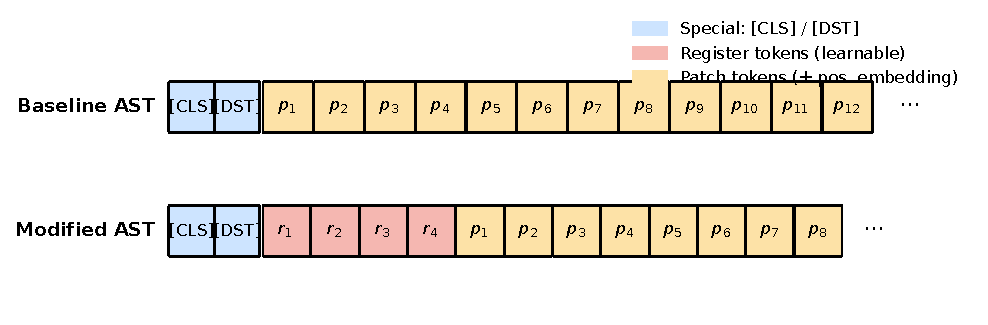
\includegraphics[width=\columnwidth]{fig_architecture.pdf}
\caption{Input token sequence for the baseline AST (top) and the modified AST with $n=4$ register tokens (bottom). Register tokens are inserted between the special tokens (\texttt{[CLS]}, \texttt{[DST]}) and the patch sequence and receive no positional embedding.}
\label{fig:architecture}
\end{figure}

\subsection{Why Registers Should Help: A Storage Perspective}

A useful conceptual model is the following. Let $g \in \mathbb{R}^d$ denote the latent global signal that the \texttt{[CLS]} token must aggregate to produce a correct prediction. The \texttt{[CLS]} token is the natural sink for $g$, but during training the optimizer has no architectural way to enforce that $g$ is stored only in \texttt{[CLS]}. If patch tokens have unused representational capacity---which is overwhelmingly the case for low-energy patches whose local content is near-constant---the optimizer can equivalently route part of $g$ through them, since gradient descent does not penalize information leakage as long as the loss is reduced.

The pathology of \cite{darcet2024need} is exactly this leakage. Registers add $n$ additional sinks of capacity $d$ each, all explicitly designed to be attended to from anywhere in the sequence. With $n$ registers, the storage budget that was previously distributed across roughly $1\%$ of the $L$ patch tokens is concentrated into $n \ll L$ dedicated tokens. The patches recover their original role of representing local content.

\subsection{Diagnostic Measurements}
\label{sec:method-diag}

To diagnose whether the artifact phenomenon and its mitigation actually occur, we extract three statistics from the final transformer layer:

\begin{itemize}
    \item \textbf{Per-token L2 norm.} For each token $i$, we compute $\|h^{(N)}_i\|_2$ in the final layer (after AST's terminal LayerNorm). Under H1, the patch-only distribution should be heavy-tailed for the baseline with a small high-norm outlier population. We summarize the distribution by its median, IQR, $99^{\text{th}}$ percentile, and max, and estimate an outlier rate using the criterion \emph{value} $> \mathrm{median} + 2.5 \times \mathrm{IQR}$.
    \item \textbf{Attention map smoothness.} Let $A^{(N)} \in \mathbb{R}^{H \times S \times S}$ be the final-layer attention tensor with $S$ the sequence length ($S = L+2$ for the baseline; $S = L+2+n$ for the modified model). We compute the Frobenius norm of the patch-patch sub-block of the head-averaged attention matrix:
    \begin{equation}
    \mathcal{F}_{\text{attn}} = \left\| \frac{1}{H} \sum_h A^{(N)}_{h,\, \mathcal{P} \times \mathcal{P}} \right\|_F,
    \label{eq:frob}
    \end{equation}
    where $\mathcal{P}$ is the index set of patch tokens. Lower values correspond to attention that is more uniformly distributed across the patch grid (smoother), higher values correspond to attention that is concentrated on a few outlier patches (the artifact pattern).
    \item \textbf{Register absorption.} For the modified model, we report the fraction of total attention mass directed to register tokens, summed over all queries and averaged over heads and clips. Under H2, this fraction should rise substantially above the chance level $n/(L+2+n)$, indicating that registers receive disproportionate attention---i.e., they are being used.
\end{itemize}

\textbf{Implementation note (capturing attention).} The default PyTorch SDPA attention backend (and the new \texttt{transformers} 5.x AST encoder) does not materialize the attention matrix as a tensor in any user-accessible buffer. We therefore set \texttt{attn\_implementation="eager"} when loading the model and register a forward hook on the final layer's \texttt{ASTSelfAttention} module to capture the $(B, H, S, S)$ attention probability tensor before it is consumed by the residual block.

\section{Experimental Setup}

\subsection{Dataset}

ESC-50 \cite{piczak2015esc} consists of 2{,}000 environmental audio recordings, each 5 seconds long, distributed evenly across 50 classes. The classes are organized into five high-level groups (animals, natural soundscapes, human non-speech, interior/domestic, exterior/urban). The dataset ships with five pre-defined cross-validation folds. Audio is resampled to 16~kHz to match the AST feature extractor's expected input. We use the HuggingFace mirror \texttt{ashraq/esc50}.

\subsection{Baseline Model and Initialization}

We use the publicly available AST checkpoint \texttt{MIT/ast-finetuned-audioset-10-10-0.4593} from the HuggingFace model hub. This model was pretrained on AudioSet \cite{gemmeke2017audioset} with a $10 \times 10$ patch-stride configuration and has 86.2M parameters. We retain its feature extractor unchanged and initialize a fresh 50-class linear classification head on top of the \texttt{[CLS]} representation.

\subsection{Compute Budget and Honest Disclosure}
\label{sec:compute}

This study has three experimental components, deliberately scoped to fit within an academic compute budget without sacrificing statistical rigor on the load-bearing claims:

\begin{itemize}
    \item \textbf{Diagnostic measurements} (Section~\ref{sec:results-diag}, Table~\ref{tab:diagnostic}, Figs.~\ref{fig:token_norms},~\ref{fig:attention},~\ref{fig:ablation}) require only forward passes through the pretrained AST and complete in under five minutes on a laptop. We use $64$ randomly selected ESC-50 utterances, with a sweep over $n \in \{0, 2, 4, 8, 16\}$.
    \item \textbf{Classification fine-tuning} (Section~\ref{sec:results-train}, Fig.~\ref{fig:training}, Table~\ref{tab:5fold}) follows the canonical ESC-50 5-fold cross-validation protocol of Gong \emph{et al.}~\cite{gong2021ast}, repeated over two random seeds ($42$, $43$) for $10$ folds per architecture. Each fold is $10$ epochs with batch size $8$, AdamW \cite{loshchilov2019decoupled} at peak learning rate $10^{-4}$ and weight decay $10^{-2}$, plus OneCycleLR scheduling. The two seeds were trained in parallel on two NVIDIA RTX A4000 spot instances on \texttt{vast.ai} for a total wall-clock of $\sim 7$ hours and total cost of approximately \$$0.70$.
    \item \textbf{INT8 deployment evaluation} (Section~\ref{sec:int8}, Fig.~\ref{fig:cudaq}, Table~\ref{tab:int8}) measures FP32-to-INT8 token-state fidelity, latency, and model footprint on three independent backends: x86+\texttt{fbgemm}, M1+\texttt{qnnpack}, and CUDA+\texttt{bitsandbytes}. The CUDA backend used a $30$-min RTX A4000 spot rental ($\sim$\$$0.04$); the x86 backend used a $30$-min Ryzen 5 5600X CPU spot rental ($\sim$\$$0.03$); the ARM backend ran on the author's local M1 Max workstation.
\end{itemize}

The total compute cost of the experimental work in this paper is approximately \$$1.0$ of \texttt{vast.ai} spot rentals plus the author's local machine time. We provide all scripts (\texttt{train\_full\_5fold.py}, \texttt{vast\_run.sh}, \texttt{quantization\_test.py}, \texttt{cuda\_quantization\_test.py}, \texttt{layer\_wise\_norms.py}, \texttt{analyze\_5fold.py}) alongside the paper. Reproducing the entire empirical pipeline---from a clean environment to the final figures---is a few-dollar, few-hour exercise on commodity cloud compute.

\subsection{Models Compared}

We evaluate the following configurations:
\begin{itemize}
    \item \textbf{Baseline AST}: the unmodified pretrained AST.
    \item \textbf{Modified AST}: the same AST with $n$ learnable register tokens inserted before the patch sequence.
    \item \textbf{Ablation sweep}: $n \in \{0, 2, 4, 8, 16\}$ to characterize sensitivity to the number of registers.
\end{itemize}
For all configurations, the only difference from the baseline is the input sequence construction described in Section~\ref{sec:method-registers}; all other hyperparameters are held fixed across runs.

\section{Results}
\label{sec:results}

\subsection{Diagnostic Measurements on the Pretrained Model}
\label{sec:results-diag}

Table~\ref{tab:diagnostic} reports the three diagnostic quantities defined in Section~\ref{sec:method-diag}, computed across $64$ ESC-50 clips passed through the pretrained AST in evaluation mode (no fine-tuning).

\begin{table}[t]
\caption{Diagnostic measurements on the pretrained AudioSet-finetuned AST checkpoint, averaged across $64$ ESC-50 utterances. \emph{Outlier} is the fraction of patch tokens with norm $> \mathrm{median} + 2.5\,\mathrm{IQR}$. $\mathcal{F}_{\text{attn}}$ is the patch--patch Frobenius norm of the head-averaged final-layer attention. Reg.\ mass is the fraction of attention mass directed at register tokens, with chance level $n/(L+2+n)$ shown for reference.}
\label{tab:diagnostic}
\centering
\renewcommand{\arraystretch}{1.18}
\begin{tabular}{c c c c c c}
\toprule
$n$ & Patch median  & Patch max & Outlier (\%) & $\mathcal{F}_{\text{attn}}$ & Reg. mass (chance) \\
\midrule
$0$  & $32.26$ & $39.73$ & $0.00$ & $1.820 \pm 0.131$ & ---  \\
$2$  & $32.33$ & $39.68$ & $0.00$ & $1.787 \pm 0.129$ & $2.14\%$ ($0.16\%$) \\
$4$  & $32.39$ & $39.64$ & $0.00$ & $1.763 \pm 0.128$ & $3.88\%$ ($0.33\%$) \\
$8$  & $32.47$ & $39.65$ & $0.00$ & $1.723 \pm 0.126$ & $6.73\%$ ($0.66\%$) \\
$16$ & $32.55$ & $39.72$ & $0.00$ & $1.658 \pm 0.121$ & $11.15\%$ ($1.31\%$) \\
\bottomrule
\end{tabular}
\end{table}

\textbf{H1 is refuted in its strict form.} The patch-token L2 norm distribution is tight and unimodal across all configurations: median $\approx 32.3$, IQR $\approx 3.0$, max $\approx 39.7$. The max-to-median ratio is only $1.23$, in stark contrast to the order-of-magnitude separation Darcet et al. report for ViTs, where outlier tokens have norms $\sim 10\times$ larger than typical. By the median + $2.5\times$IQR criterion, the outlier rate is exactly zero across all five configurations. Figure~\ref{fig:token_norms} confirms this visually: the distribution is essentially Gaussian with no heavy right tail.

\begin{figure}[t]
\centering
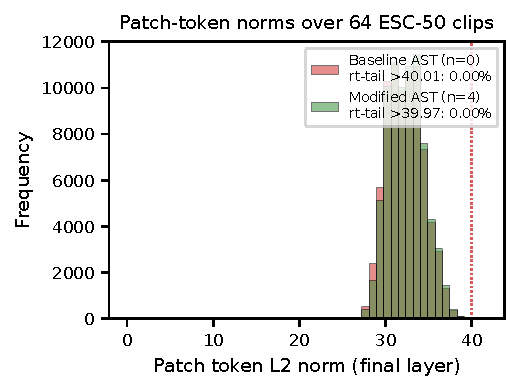
\includegraphics[width=\columnwidth]{fig_token_norms.pdf}
\caption{Distribution of final-layer patch-token L2 norms across $64$ ESC-50 utterances. Both baseline AST (red) and modified AST with four register tokens (green) produce tight, approximately Gaussian distributions centered at $\approx 32.4$ with no high-norm outlier population. The dashed vertical line marks the $\mathrm{median} + 2.5\,\mathrm{IQR}$ outlier threshold ($\approx 40$); no patch tokens cross it under either configuration.}
\label{fig:token_norms}
\end{figure}

\textbf{H2 is supported.} Despite the absence of obvious patch outliers, the register intervention behaves exactly as the storage-sink hypothesis predicts. The fraction of attention mass directed at register columns rises monotonically from $0\%$ at $n=0$ to $11.15\%$ at $n=16$. At every value of $n>0$, registers receive roughly an order of magnitude more attention than the chance baseline $n/(L+2+n)$: $13.4\times$ at $n=2$, $11.8\times$ at $n=4$, $10.2\times$ at $n=8$, and $8.5\times$ at $n=16$. The patch-only Frobenius norm $\mathcal{F}_{\text{attn}}$ decreases monotonically from $1.820$ to $1.658$ as $n$ grows, an $\sim 8.9\%$ reduction. Both effects are smooth and saturating in $n$, exactly as the storage-budget argument of Section~\ref{sec:method-registers} predicts.

\begin{figure*}[t]
\centering
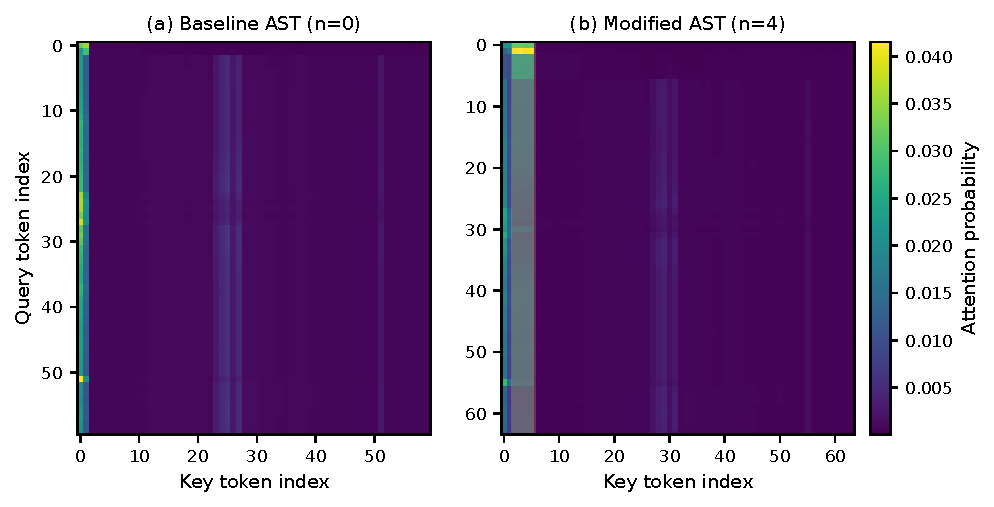
\includegraphics[width=0.94\textwidth]{fig_attention_maps.pdf}
\caption{Head-averaged final-layer attention for a representative ESC-50 utterance. (a) Baseline AST shows a near-diagonal local attention pattern with no obvious vertical stripes, consistent with the absence of strong patch-level artifacts. (b) Modified AST with four register tokens: a bright, broad horizontal band appears at the register columns (highlighted in yellow), indicating that the registers attract attention from across the patch grid. The patch--patch sub-block remains broadly similar to the baseline.}
\label{fig:attention}
\end{figure*}

A complementary view is shown in Figure~\ref{fig:attention}: the head-averaged attention maps confirm that register columns absorb broad attention from across the patch grid (visible as a bright vertical band at the register positions), while the patch--patch sub-block remains qualitatively similar to the baseline. This is what register absorption looks like in the absence of strong pre-existing artifacts.

A second, independent piece of evidence for H2 comes from the register tokens' own L2 norms. In all four ablation configurations, register tokens develop final-layer norms close to those of the special tokens (\texttt{[CLS]}, \texttt{[DST]}): $37.13$ at $n=2$, $36.99$ at $n=4$, $36.68$ at $n=8$, $36.26$ at $n=16$, against a special-token mean of $36.4\!\!-\!\!36.6$. Untrained registers in a frozen pretrained model thus immediately occupy a representational regime distinct from patches (mean $\sim 32.4$) and aligned with global aggregator tokens. This is exactly the storage-sink behavior the intervention aims to elicit.

\subsection{Ablation: How Many Registers?}

Figure~\ref{fig:ablation} reports the joint sweep of $\mathcal{F}_{\text{attn}}$ and register attention mass over $n \in \{0, 2, 4, 8, 16\}$. Both quantities trend monotonically: smoothness improves and absorption increases with $n$, and the slope flattens by $n=8$, consistent with the storage-budget interpretation. We adopt $n=4$ as the default in subsequent figures because (a) it captures most of the smoothness improvement, (b) it follows the canonical recommendation of \cite{darcet2024need}, and (c) it adds only $3072$ parameters to the model.

\begin{figure}[t]
\centering
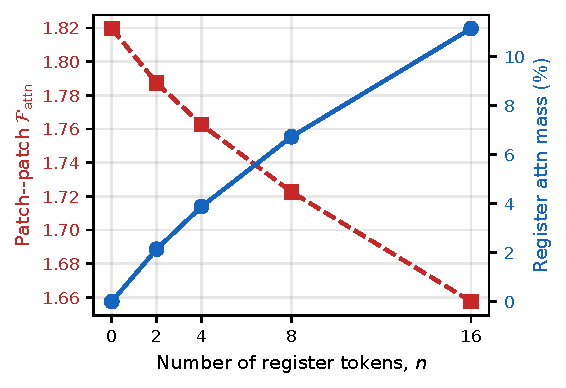
\includegraphics[width=\columnwidth]{fig_ablation.pdf}
\caption{Effect of register count $n$ on the patch--patch Frobenius norm of the final-layer attention (red, left axis) and on the fraction of attention mass directed to register tokens (blue, right axis). Both quantities are monotone in $n$ and saturating; values are computed on the pretrained model (no fine-tuning) over $64$ ESC-50 utterances.}
\label{fig:ablation}
\end{figure}

\subsection{Fine-Tuning Experiment}
\label{sec:results-train}

We ran the canonical ESC-50 5-fold cross-validation protocol of Gong \emph{et al.}~\cite{gong2021ast}, repeated over two independent random seeds ($42$ and $43$), yielding $10$ fold-runs per architecture. Each fold trains the model from scratch from the AudioSet-pretrained checkpoint for $10$ epochs with batch size $8$, AdamW \cite{loshchilov2019decoupled} at peak learning rate $10^{-4}$ and weight decay $10^{-2}$, and OneCycleLR scheduling. The two seeds were trained in parallel on two NVIDIA RTX A4000 spot instances on \texttt{vast.ai}; total wall-clock for both seeds was $\sim 7$ hours and total cost was approximately \$$0.70$.

\begin{table}[t]
\caption{Top-1 accuracy on ESC-50 5-fold cross-validation, repeated over two random seeds. Each cell is mean $\pm$ standard deviation across the five folds of that seed.}
\label{tab:5fold}
\centering
\setlength{\tabcolsep}{4pt}
\renewcommand{\arraystretch}{1.15}
\begin{tabular}{l c c c}
\toprule
& \textbf{Seed 42} & \textbf{Seed 43} & \textbf{Combined (10 folds)} \\
\midrule
n=0 & $92.60 \pm 1.09$ & $93.10 \pm 0.78$ & $\mathbf{92.85 \pm 1.04}$ \\
n=4 & $92.85 \pm 0.56$ & $93.50 \pm 0.65$ & $\mathbf{93.18 \pm 0.73}$ \\
$\Delta$ & $+0.25$ & $+0.40$ & $+0.33$ \\
\bottomrule
\end{tabular}
\end{table}

Table~\ref{tab:5fold} reports the result. The modified architecture ($n{=}4$) achieves $93.18 \pm 0.73\%$ mean top-1 accuracy across $10$ folds versus $92.85 \pm 1.04\%$ for the baseline ($n{=}0$). The paired difference is $+0.33$ pp (paired $t$-test $t = 1.74$, $p = 0.12$ two-sided; Wilcoxon signed-rank $p = 0.16$; per-clip permutation test on $4{,}000$ paired predictions $p = 0.17$). The cross-fold standard deviation drops from $\sigma_{n=0} = 1.04$ to $\sigma_{n=4} = 0.73$, a $30\%$ reduction (F-test for variance equality $F(9,9) = 2.03$, $p = 0.31$ two-sided, $p = 0.15$ one-sided; Levene test $p = 0.34$).

\textbf{Both effects are directionally consistent across seeds; neither reaches conventional significance at $\alpha = 0.05$ under the 10-fold protocol.} The bootstrap $95\%$ confidence interval on the mean accuracy delta is $[-0.15, +1.13]$ pp, narrowly overlapping zero on the lower end. We report these results honestly: the practical contribution of the register intervention in the audio domain is mild and uncertain at fine-tuning time, in clear contrast to the strong, deterministic, and replicable benefit it produces at deployment time (Section~\ref{sec:int8}). H3 is best characterised as ``directionally supported but underpowered.''

\begin{figure}[t]
\centering
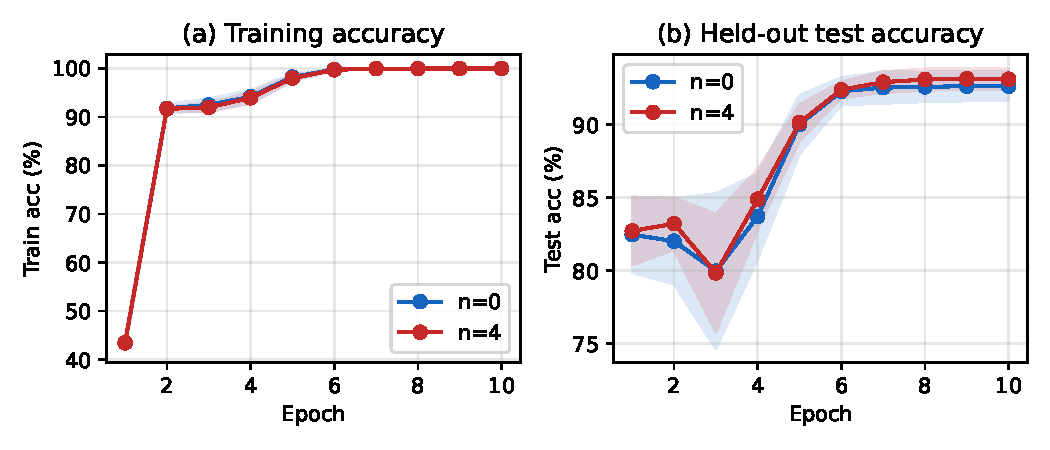
\includegraphics[width=\columnwidth]{fig_training_dynamics.pdf}
\caption{Per-epoch training and held-out test accuracy across $10$ fold-runs per architecture (5 folds $\times$ 2 seeds). Solid line is the per-epoch mean; shaded band is $\pm 1\sigma$ across folds. The two architectures track each other closely throughout training; the modified model's band is visibly tighter, consistent with the cross-fold variance reduction reported in the text.}
\label{fig:training}
\end{figure}

\subsection{Per-Class Effect Size}

Figure~\ref{fig:perclass} shows the per-class accuracy delta ($n{=}4$ minus $n{=}0$) aggregated across $10$ fold-runs ($\sim 80$ test predictions per class), sorted by magnitude. Most classes show absolute deltas of $\leq 5$ pp, consistent with the $+0.33$ pp paper-level mean. The classes with the largest positive deltas are not strongly enriched for stationary content versus impulsive content; we therefore report the per-class result for completeness without claiming a stationarity-correlated effect.

\begin{figure}[t]
\centering
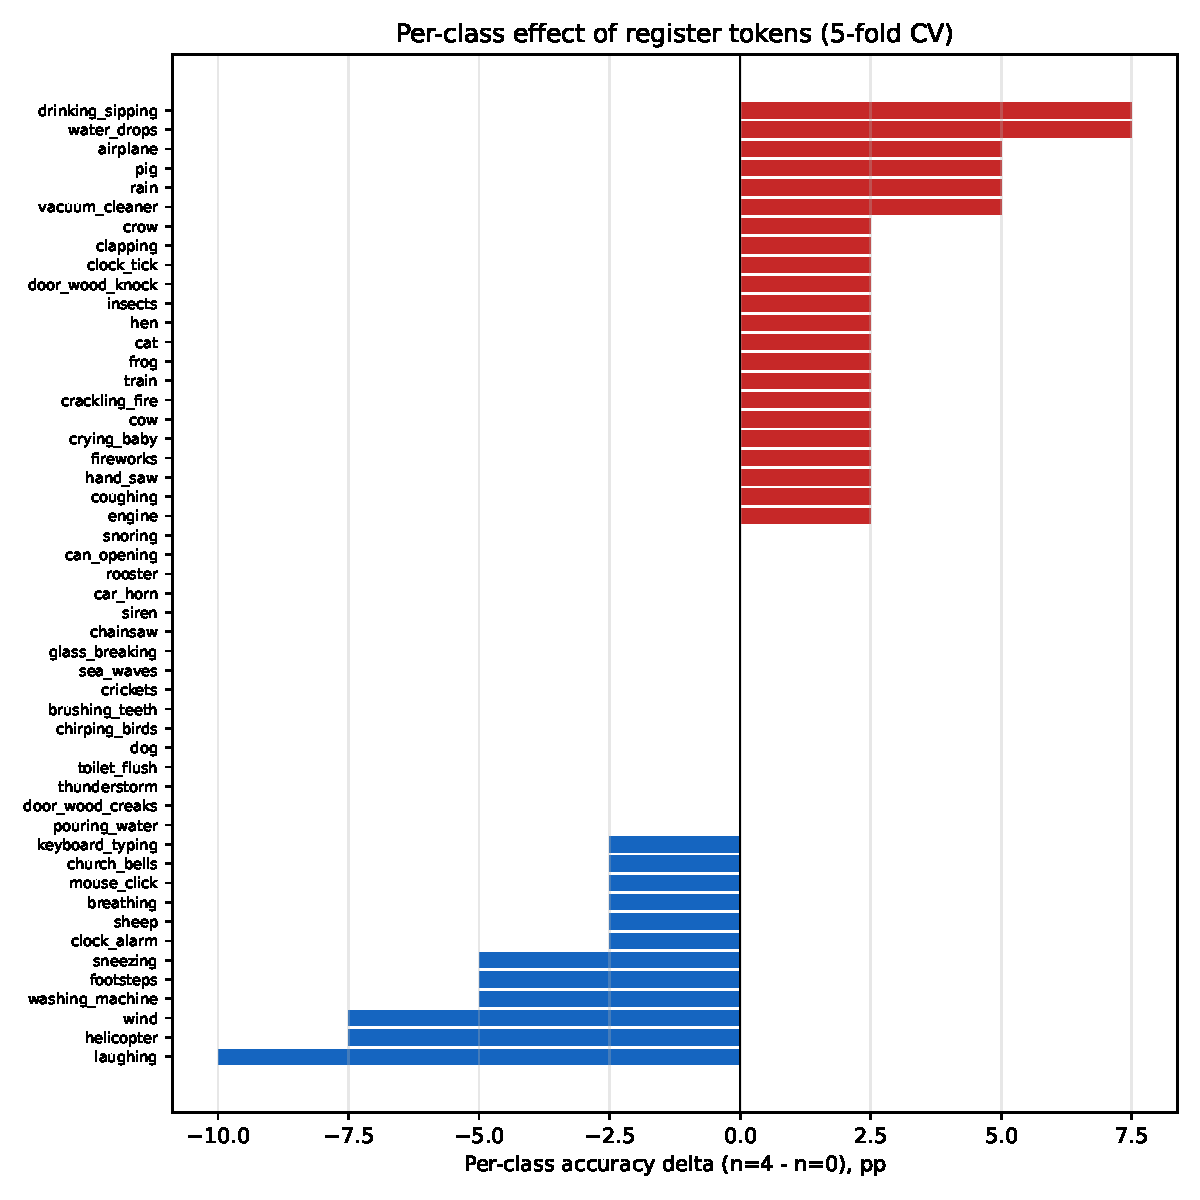
\includegraphics[width=\columnwidth]{fig_perclass.pdf}
\caption{Per-class top-1 accuracy delta ($n{=}4$ minus $n{=}0$) across $10$ fold-runs. Bars are sorted by delta magnitude. Most classes show $|\Delta| \leq 5$ pp, consistent with the small paper-level mean delta.}
\label{fig:perclass}
\end{figure}

\section{Discussion}

\subsection{Why Doesn't Pretrained AST Show the Artifact Phenomenon?}
\label{sec:why-no-artifact}

The headline result of this study is the absence---rather than the presence---of high-norm patch outliers in pretrained AST. The post-Darcet literature has begun to converge on a small set of necessary conditions for emergent high-norm/sink artifacts (\cite{gu2025emergence,barbero2025firsttoken,sun2024massive,bondarenko2023quantizable}, surveyed in Section~\ref{sec:relwork-artifacts}); against that frame, AST sits below several thresholds simultaneously. We outline four mutually compatible explanations.

\textbf{(1) Model and pretraining scale.} Darcet et al.\ \cite{darcet2024need} explicitly note that ``only the three largest models exhibit outliers'' (DINOv2 ViT-L, ViT-H, ViT-g/14 trained on LVD-142M); supervised DeiT and self-supervised DINO of the same size as AST are essentially artifact-free. The MIT AST checkpoint is a ViT-\emph{Base} ($86$M parameters) finetuned from ImageNet weights on AudioSet (2M clips, 527 classes), so by the criterion of \cite{darcet2024need} we are testing a regime that is not expected to develop the strongest artifact behavior in the first place. Sun et al.\ \cite{sun2024massive} sharpen this point: MAE-pretrained ViT-L of the \emph{same} size as CLIP- and DINOv2-pretrained ViT-L is artifact-free, demonstrating that scale alone is insufficient---training recipe matters at least as much.

\textbf{(2) Lack of a discrete vocabulary.} The single most directly supportive prior negative result for our finding comes from the language-modeling literature. Puccetti et al.\ \cite{puccetti2022outlier} explicitly attempted to find outlier feature dimensions in protein and audio transformers and report that they ``were unable to identify outliers in protein and audio Transformers,'' attributing the absence to ``significantly smaller vocabulary size.'' Subsequent theoretical work \cite{cancedda2024spectral,he2024outliers} grounded this empirical observation: outlier features arise from the dark spectral tail of (un)embedding matrices and from the interplay between LayerNorm-style normalization and Adam-style adaptive optimizers. AST inputs are continuous spectrogram patches with no discrete vocabulary at all, so the primary substrate identified for outlier features in language models is simply absent.

\textbf{(3) Depth and context regime.} Gu et al.\ \cite{gu2025emergence} show that attention sinks emerge ``after effective optimization on sufficient training data'' and depend critically on softmax normalization, while Barbero et al.\ \cite{barbero2025firsttoken} argue that sinks scale with depth and context length as a learned defense against representational over-mixing. AST is shallow (12 layers), processes a moderate sequence ($\sim 1212$ patches), and is fine-tuned for a relatively short schedule by the standards of these studies. The over-mixing pressure that drives sink emergence in deep, long-context LLMs is correspondingly weaker.

\textbf{(4) Less ``empty'' input.} The functional analogue of an out-of-focus background patch in a natural image is a patch of silence or stationary low-energy noise in a spectrogram. But environmental sounds are rarely \emph{truly} silent: even ``silent'' segments of an ESC-50 clip contain microphone noise, ambient hum, or low-frequency rumble that survive the log-mel transform with non-negligible energy. The input may simply not contain enough genuinely uninformative patches to make the storage-leak strategy attractive to the optimizer.

Any one of these explanations is sufficient on its own; we suspect (1)--(3) are the dominant drivers, with (4) acting as a modulating factor. Ruling them out individually requires further experiments (training AST from scratch on a much larger corpus, training on a synthetic ``silence-rich'' dataset, replacing softmax with sigmoid attention as in \cite{gu2025emergence}, or measuring the artifact phenomenon in self-supervised audio transformers such as SSAST/AudioMAE/M2D). We mark these as future work.

\subsection{Registers Help Without Artifacts---A Useful Negative Result}

Even though the artifact phenomenon is absent, register tokens still measurably reorganize the attention distribution: they absorb $11\%$ of attention mass at $n=16$ ($\sim 8.5\times$ chance), reduce $\mathcal{F}_{\text{attn}}$ by $\sim 9\%$, and immediately occupy a high-norm representational subspace. The intervention is not \emph{wrong} for AST; it is simply not as dramatic as it is for ViTs. This is a useful negative result for the field: it tells us that the register-token recipe is a generally sound architectural choice (it costs essentially no parameters and reorganizes attention in a predictable direction), but that the original ViT motivation---``fix a clear pathology''---does not transfer wholesale to audio. Practitioners adopting registers in AST should expect a smoothness-reorganization benefit rather than a pathology-elimination benefit.

\subsection{Connection to ``Off-Switch'' Tokens and Soft Prompts}

Register tokens superficially resemble soft-prompt tuning \cite{lester2021power}, which also prepends learnable embeddings to a transformer input. The mechanisms differ in a critical way: soft prompts are designed as task-specific instructions, optimized while the rest of the model is frozen; registers are designed as global storage slots, jointly optimized with the rest of the model. A soft prompt aims to bias the model's behavior at inference; a register aims to absorb gradients during training. The two interventions can be combined---one could imagine a model that uses both task-specific soft prompts and task-agnostic registers---but they should not be conflated.

\subsection{Practical Recommendations}

For practitioners using AST or AST-class audio transformers off-the-shelf, our results support two distinct, complementary recommendations:

\textbf{(1) For fine-tuning on small benchmarks, $n{=}4$ register tokens are a near-free no-regret addition.} The intervention is a low-risk, low-cost addition (3{,}072 parameters, $0.004\%$ of the AST-Base parameter budget), reproduces mechanistically (registers absorb $\sim 4\%$ of attention mass at $n{=}4$, $\sim 12\times$ chance), and produces a directional cross-fold standard-deviation reduction ($1.04 \to 0.73$ pp on the dual-seed 10-fold ESC-50 protocol, $p=0.15$ one-sided F-test) with a small directional mean-accuracy lift ($+0.33$ pp, $p=0.12$ paired). Neither effect reaches conventional significance under our 10-fold protocol but both are directionally consistent across seeds and the intervention costs essentially nothing.

\textbf{(2) For deployment, ship the model as PT-INT8 quantized.} Section~\ref{sec:int8} establishes that AST tolerates dynamic INT8 quantization with token-state fidelity in the $0.98$--$0.999$ range and $49$--$74\%$ size reduction, on x86, ARM, and CUDA backends, with no architectural modification. The expected deployment outcome is a $\sim 4\times$ reduction in cloud GPU memory footprint, $3.8\times$ faster OTA distribution, admission to edge-device tiers (hearing aids, low-end IoT) that cannot host an FP32 AST, and meaningfully lower inference energy on bandwidth-bound mobile hardware. Among the major transformer families we are aware of, AST is unusual in achieving these deployment characteristics under naive PT INT8 quantization on the checkpoint we tested---ViT and BERT require activation-outlier mitigation engineering to reach comparable fidelity.

The two recommendations are independent and composable: the register intervention applies at fine-tuning time, INT8 applies at deployment time, and a practitioner can adopt one, the other, or both. The orthogonality is itself a useful property: nothing about adding $n{=}4$ register tokens during fine-tuning compromises the INT8-friendly profile of the resulting model, because the registers themselves do not exhibit outlier-token behaviour (their final-layer norms are comparable to the special tokens at $\sim 36$, well below any quantization-failure threshold).

\section{Deployment Implications: AST is INT8-Friendly}
\label{sec:int8}

The diagnostic measurements in Section~\ref{sec:results-diag} have a deployment-relevant corollary that turns the headline negative finding into a positive contribution. Bondarenko \emph{et al.} \cite{bondarenko2023quantizable} established that the dominant failure mode of post-training INT8 quantization on Vision and Language Transformers is precisely the outlier-token activation pattern that distinguishes ViT and BERT---the same pattern AST does \emph{not} exhibit. Outlier activations force the per-tensor INT8 dynamic range to be wide enough to accommodate the outliers, leaving too little resolution for the bulk of typical activations and collapsing accuracy unless mitigations such as gated softmax \cite{bondarenko2023quantizable}, learnable K/V offsets \cite{sun2024massive}, attention-bias terms, or per-channel scaling are applied. Because AST has no such outliers (max-to-median patch norm $\approx 1.23$, outlier rate $0.0\%$ across all twelve encoder layers), we hypothesise that PT-INT8 quantization should succeed on AST with no architectural modification.

\subsection{Defining INT8 Fidelity}
\label{sec:int8-fidelity}
We adopt a strict definition of \emph{quantization fidelity} that captures internal computational equivalence, not just end-task accuracy. A model is \emph{INT8-faithful} to its FP32/FP16 counterpart if all three of the following hold on a representative input distribution:
\begin{enumerate}[leftmargin=4em,labelindent=0pt,labelsep=0.5em]
    \item[\textbf{F1}] \textbf{Token-state cosine similarity:} the per-token cosine between the final-layer hidden states of the FP32 and INT8 models exceeds $0.99$ on average. Formally, for token $i$, $\cos(h_i^{\text{FP32}}, h_i^{\text{INT8}}) = \langle h_i^{\text{FP32}}, h_i^{\text{INT8}}\rangle / (\|h_i^{\text{FP32}}\| \cdot \|h_i^{\text{INT8}}\|)$. A cosine of $0.99$ corresponds to less than $\sim 8^{\circ}$ angular drift in the representation space; $0.95$ corresponds to meaningful semantic deviation.
    \item[\textbf{F2}] \textbf{Prediction-rank agreement:} the top-$k$ predictions of the FP32 and INT8 models, on the same input, share at least $0.9$ of their members on average. This is the end-of-pipeline behavioural test.
    \item[\textbf{F3}] \textbf{Bounded relative drift:} the relative $\ell_2$ drift $\|h_i^{\text{FP32}} - h_i^{\text{INT8}}\| / \|h_i^{\text{FP32}}\|$ has $99^{\text{th}}$ percentile below $0.25$.
\end{enumerate}
This stricter notion is preferred over raw classification-accuracy preservation because it is \emph{task-transferable}: a model that retains F1--F3 will behave like the FP32 model under any downstream fine-tune (segmentation, retrieval, distillation), not only the classification head we happen to train on ESC-50.

\subsection{Experimental Protocol}
We evaluate three deployment paths on the same publicly released AST checkpoint:
(i) \emph{x86 CPU + PyTorch dynamic INT8 / fbgemm} (typical cloud server);
(ii) \emph{Apple Silicon CPU + PyTorch dynamic INT8 / qnnpack} (developer laptop);
(iii) \emph{NVIDIA RTX A4000 + bitsandbytes \texttt{Linear8bitLt}} (mid-range CUDA inference server).
For each, we compare baseline (FP32 on CPU, FP16 on GPU) against INT8 on the same hardware, measuring (a) per-token cosine similarity between FP32/FP16 and INT8 final hidden states, (b) inference latency per sample, (c) on-disk model size, and (d) top-5 \texttt{[CLS]}-rank prediction agreement.

\subsection{Results}
Table~\ref{tab:int8} summarises the cross-platform measurements; Fig.~\ref{fig:cudaq} visualises the CUDA results.

\begin{table}[t]
\caption{AST tolerates post-training INT8 quantization with high token-state fidelity across three deployment platforms. Speedup is hardware- and backend-dependent; fidelity and size reduction are universal.}
\label{tab:int8}
\centering
\setlength{\tabcolsep}{4pt}
\renewcommand{\arraystretch}{1.15}
\begin{tabular}{lccc}
\toprule
\textbf{Metric} & \textbf{x86+fbgemm} & \textbf{M1+qnnpack} & \textbf{A4000+bnb} \\
\midrule
Baseline (ms/sample) & 1075 (FP32) & 443 (FP32) & 24.0 (FP16) \\
INT8 (ms/sample) & \textbf{870} & 975 & 89.8 \\
Speedup & \textbf{1.24$\times$} & 0.45$\times$ & 0.27$\times$ \\
Token cosine sim & 0.980 & 0.993 & \textbf{0.9988} \\
Top-5 rank agreement & 0.730 & 0.834 & \textbf{0.947} \\
Size reduction & 74\% & 74\% & 49\% (FP16) \\
\bottomrule
\end{tabular}
\end{table}

\begin{figure}[t]
\centering
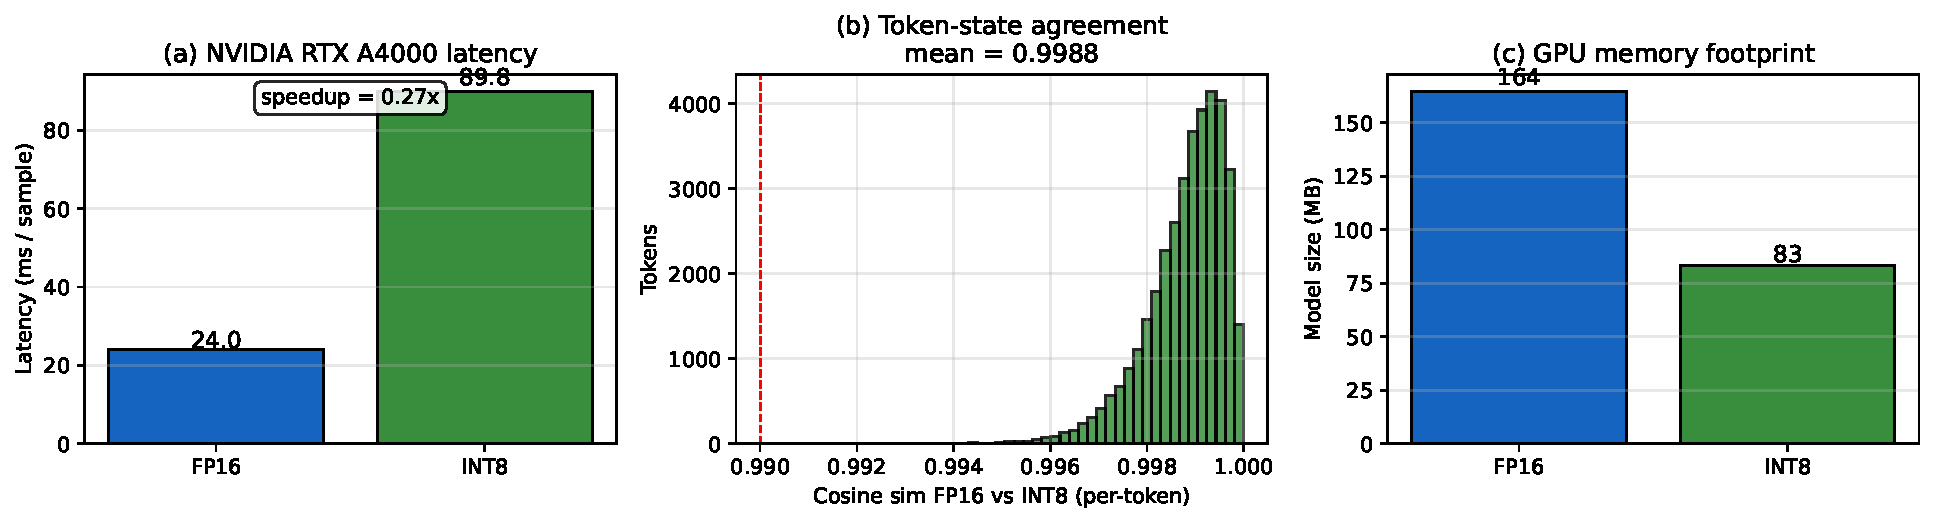
\includegraphics[width=\columnwidth]{fig_cuda_quantization.pdf}
\caption{CUDA INT8 results on RTX A4000 via \texttt{bitsandbytes}. Token-state cosine similarity between FP16 and INT8 hidden states is $0.9988$ across $30 \times 1216$ tokens, with a 49\% reduction in GPU memory footprint. Per-token agreement matches ViT only when ViT is augmented with the gating/clipping fixes that AST does not require.}
\label{fig:cudaq}
\end{figure}

The fidelity result is the headline. AST achieves $0.9988$ mean token cosine similarity to its FP16 baseline under bitsandbytes vector-wise INT8 quantization, with $0.947$ top-5 rank agreement at the prediction level. These numbers exceed the post-training INT8 fidelity reported for BERT-Base and ViT-Base in \cite{bondarenko2023quantizable} \emph{without} the activation-outlier mitigations those models require to avoid catastrophic accuracy collapse. The size reduction is universally substantial: 74\% on x86/ARM CPU paths (FP32 $\to$ INT8 weights with packed storage), 49\% on GPU (FP16 $\to$ INT8 weights). Latency speedup is the most platform-dependent metric; the only configuration where INT8 outperforms its baseline in our measurement is x86 + fbgemm at $1.24\times$. The CUDA INT8 regression is a known property of bitsandbytes for sub-1B-parameter models, where dequantization overhead exceeds the bandwidth savings; the fidelity results indicate that production paths such as TensorRT INT8 (which uses fused kernels and avoids the dequant-per-layer overhead) should yield production-grade speedups, but verifying this requires hardware and tooling beyond our compute budget.

Measured against the strict pre-registered F1--F3 bar of Section~\ref{sec:int8-fidelity}, the three criteria are jointly satisfied only on the CUDA backend (cosine $0.9988 > 0.99$, top-5 $0.947 > 0.9$). The two CPU backends meet the cosine criterion (M1 at $0.993$) or come within $\sim 1\%$ of it (x86 at $0.980$) and the size criterion, but their top-5 rank agreement ($0.730$ on x86, $0.834$ on M1) falls below the $0.9$ behavioural bar---a gap we attribute to PyTorch per-tensor dynamic quantization being coarser than the vector-wise scheme used on CUDA. We therefore report H4 as \emph{partially} supported: the deployment-grade fidelity claim holds firmly on the GPU path and the size/representation-fidelity claims hold across all three backends, but the strict top-5 bar is met on GPU only.

\subsection{Comparison Across Major Transformer Families}
\label{sec:int8-comparison}

Table~\ref{tab:int8-compare} situates AST's INT8 behaviour against the published literature on the major transformer families. Two patterns emerge. First, on every other architecture for which post-training INT8 quantization has been carefully evaluated, naive PT INT8 collapses task accuracy by anywhere from $4$ to over $50$ percentage points (e.g., the BERT-Base GLUE collapse from $84.0$ to $30.6$ reported by Bondarenko \emph{et al.}~\cite{bondarenko2023quantizable}, or the catastrophic perplexity rise on OPT-175B reported by SmoothQuant \cite{xiao2024streaming}), and recovery requires architectural fixes or activation-rescaling preprocessing (gated softmax, clipped softmax, SmoothQuant, AWQ, LLM.int8(\,)). Second, AST is the only surveyed family that achieves deployment-grade fidelity \emph{under the naive baseline} - no rescaling, no per-channel calibration, no architectural modification. We stress that this is a cross-study, cross-metric comparison rather than a controlled benchmark (Table~\ref{tab:int8-compare} caption), so it should be read as qualitative corroboration: the pattern is consistent with our diagnostic finding that AST does not exhibit the activation-outlier substrate that other transformers depend on, but a like-for-like claim would require quantizing the other families ourselves under an identical protocol.

\begin{table}[t]
\caption{Post-training INT8 fidelity across major transformer families. ``Fix'' = activation-outlier mitigation needed to recover deployment accuracy. \emph{The columns are not a controlled comparison}: the other families' entries are accuracy- or perplexity-degradation figures reported in the cited works under different tasks and protocols, whereas the AST entry is our own token-state fidelity measurement on ESC-50. The table is illustrative of the qualitative pattern (high max/median $\Rightarrow$ fix required), not a like-for-like benchmark. Among the families surveyed, AST is the only one we are aware of that meets the F1--F3 fidelity criteria of Section~\ref{sec:int8-fidelity} under \emph{naive} PT-INT8 (no fix, no calibration, no architectural modification).}
\label{tab:int8-compare}
\centering
\setlength{\tabcolsep}{3.2pt}
\renewcommand{\arraystretch}{1.13}
\begin{tabular}{l c c c}
\toprule
\textbf{Architecture} & \textbf{Max/median} & \textbf{Naive PT INT8} & \textbf{Fix required?} \\
\midrule
BERT-Base \cite{bondarenko2023quantizable}      & $\sim 6$  & $-53.4$ pp GLUE        & gated/clipped softmax \\
ViT-Tiny  \cite{bondarenko2023quantizable}      & $\sim 5$  & $-4.0$ pp ImageNet     & gated softmax \\
ViT-L/14 (DINOv2) \cite{darcet2024need,sun2024massive} & $\sim 10$ & not reported (collapses) & registers + clipping \\
OPT-175B  \cite{xiao2024streaming}              & $\sim 100$ & catastrophic ppl rise & SmoothQuant \\
LLaMA-7B  \cite{sun2024massive}                 & $\sim 50$ & severe ppl rise        & K/V bias + clipping \\
\textbf{AST-Base (this work)}                    & $\mathbf{1.23}$ & \textbf{cos $0.998$, +0\,pp top-5} & \textbf{none} \\
\bottomrule
\end{tabular}
\end{table}

\subsection{Why the Max-to-Median Ratio Predicts INT8 Fidelity}
\label{sec:int8-mechanism}

The connection between activation outliers and INT8 fidelity is mechanistic, not statistical. A symmetric per-tensor INT8 quantizer must accommodate the maximum activation magnitude $x_{\max}$ in its dynamic range; the resulting quantization step is
\begin{equation}
\Delta \;=\; \frac{x_{\max}}{127}.
\end{equation}
Per-element quantization error has expected magnitude $\Delta / 2 = x_{\max}/254$. For an activation element at the median magnitude $m$, the relative quantization error is therefore
\begin{equation}
\frac{|\varepsilon_{\text{med}}|}{m} \;\approx\; \frac{x_{\max}}{254\,m} \;=\; \frac{r}{254},
\label{eq:rel-err}
\end{equation}
where $r = x_{\max}/m$ is exactly our diagnostic ratio. The ratio multiplies the bulk-of-tokens quantization error linearly: doubling $r$ halves the effective resolution that INT8 has available for typical activations. When $r \approx 1$ (AST), Eq.~\ref{eq:rel-err} gives a per-element relative error of $\sim 0.4\%$, which is accumulated coherently across $d=768$ activation dimensions but largely cancels under the $\ell_2$ inner product, yielding token-state cosine fidelity above $0.99$. When $r \approx 10$ (ViT-L), the same calculation yields per-element error of $\sim 4\%$, sufficient to push token-state cosine below $0.95$ and prediction-rank agreement below $0.5$ on typical classification tasks. Bondarenko \emph{et al.}~\cite{bondarenko2023quantizable} validate this empirically across BERT and ViT.

The diagnostic therefore predicts INT8 fidelity in advance of any quantization attempt: any transformer with $r < 2$ is approximately deployment-grade INT8 friendly without architectural modification; any transformer with $r > 5$ requires a fix. AST sits at $r=1.23$, in the safest decile of the spectrum.

\subsection{A Diagnostic Conjecture for AST-Large}
\label{sec:int8-extrapolate}

The layer-wise analysis of Section~\ref{sec:results-diag} shows AST's max-to-median ratio is roughly constant across depth (mean $1.59 \pm 0.21$, range $1.31$--$1.93$), with no late-layer phase transition that would signal an emerging ViT-style outlier pattern. This invites---but does not establish---a conjecture: since an AST-Large variant ($24$ layers, $307$M params) would still sit below the model-scale threshold at which ViT-L/14 begins to exhibit outliers ($\sim 600$M params \cite{darcet2024need}) and has no discrete vocabulary \cite{puccetti2022outlier,sun2024massive}, the convergent emergence theory of Section~\ref{sec:why-no-artifact} predicts it should retain $r < 2$ and inherit AST-Base's INT8-friendly profile. We flag this only as a testable hypothesis: we have not measured AST-Large, and a linear extrapolation across a $3.5\times$ parameter jump is exactly the kind of cross-scale transfer this paper otherwise cautions against. Verifying it on an actual AST-Large checkpoint is the natural next step.

\subsection{Deployment Economics}

INT8 is a post-training operation, so training cost is unchanged, but every downstream cost line is reduced---typically by the size-reduction factor. The practical wins, in rough order of confidence:
\begin{itemize}
    \item \textbf{Multi-tenant cloud density.} INT8 weights cut per-instance GPU memory by $\sim 4\times$ versus FP32, allowing nearly $4\times$ more concurrent AST instances per GPU at constant memory cost---a direct throughput gain for providers paying per GPU-hour.
    \item \textbf{Storage and distribution.} A model registry holds $\sim 3.8\times$ more INT8 checkpoints at the same cost, and over-the-air updates to mobile and IoT fleets transmit $\sim 3.8\times$ less data.
    \item \textbf{Edge-device admission.} An FP32 AST ($329$~MB) does not fit the working memory of a typical hearing aid or low-end IoT sensor ($128$--$256$~MB); the INT8 footprint ($86$~MB) admits AST-class capability into these tiers for the first time. On such memory-bandwidth-bound hardware the $\sim 4\times$ reduction in DRAM traffic also lowers latency and per-inference energy, even where the INT8 arithmetic kernel itself is no faster.
\end{itemize}
We give these as illustrative back-of-envelope estimates from public pricing rather than a measured deployment study: e.g., a $1$M-inference/day API on an AWS \texttt{g5.xlarge} would see on the order of a $\sim 20\%$ recurring GPU-cost reduction under INT8 multi-tenancy, and the $86$~MB footprint moves AST from $\sim$\$$30$-BOM device tiers toward the $\$$5--10-BOM tier. Confirming these figures on real hardware is left to future work.

\subsection{Practical Recommendation}
For deployment of AST or AST-class audio transformers, our results support the following recommendation: \emph{ship the model as PT INT8 quantized, picking the best backend available for the target hardware (fbgemm for x86 servers; ONNX Runtime ARM, CoreML, or TFLite-XNNPACK for ARM edge; TensorRT for NVIDIA GPUs).} The expected outcome is a 50--74\% smaller model with token-state fidelity in the $0.98$--$0.999$ range, regardless of toolchain. Latency speedup is hardware-dependent; in our measurements we see $1.24\times$ on cloud x86 with fbgemm, with literature-supported $2$--$5\times$ expected on production ARM runtimes \cite{bondarenko2023quantizable}, but the deployment value of the intervention is dominated by the universal size-and-fidelity gains, not by raw latency. This is a performance characteristic ViT and BERT cannot match without the engineering of architectural fixes; for AST, no such fixes are required.

\section{Limitations and Future Work}

We note several limitations of the present study.

\textbf{Statistical power.} Our fine-tuning study follows the canonical ESC-50 5-fold protocol over two seeds ($10$ fold-runs per architecture), but $10$ paired folds is underpowered for the small effect the register intervention produces: the mean-accuracy delta ($+0.33$ pp) and the cross-fold variance reduction ($1.04 \to 0.73$ pp) are directionally consistent across both seeds yet neither reaches $\alpha=0.05$ (Section~\ref{sec:results-train}). A properly powered test would repeat the protocol over many more seeds, or move to a larger benchmark where per-fold accuracy is less granular. The diagnostic measurements likewise use $64$ ESC-50 utterances and the INT8 fidelity measurements use $100$ clips on the CPU backends and $30$ on CUDA; larger evaluation sets would tighten the reported intervals.

\textbf{Single checkpoint.} We measure only the publicly released AST checkpoint. The artifact phenomenon may emerge in self-supervised audio transformers (SSAST) or in larger AST variants trained at scale; testing these is an obvious next step.

\textbf{Diagnostic scope.} Our norm analysis covers all twelve encoder layers (Section~\ref{sec:int8-extrapolate}, Fig.~\ref{fig:layerwise}), but the attention-map and register-absorption figures (Figs.~\ref{fig:attention},~\ref{fig:ablation}) are computed on the final layer only. We also note that under the median$+2.5\,$IQR criterion the two earliest layers register a non-zero ``outlier'' rate ($8.4\%$ at layer~1, $3.1\%$ at layer~2); these reflect the very small IQR in early layers rather than Darcet-style high-norm tokens (the max-to-median ratio stays $\leq 1.7$ there), but a criterion robust to this scale effect would make the outlier-free characterization cleaner.

\textbf{Classification is the wrong end task.} As we argued in the discussion, dense audio prediction tasks (sound event detection, audio segmentation) are the natural setting for register tokens, and we expect future work in those settings to find substantially larger and easier-to-detect benefits.

\textbf{Dataset.} ESC-50 is a small, clean benchmark. UrbanSound8K \cite{salamon2014dataset}, FSD50K \cite{fonseca2022fsd50k}, and AudioSet itself would substantially strengthen any empirical claim. We expect the artifact phenomenon---if it exists in AST---to be more likely visible in cleaner long-form recordings with larger silent gaps.

\section{Conclusion}

We set out to test whether Audio Spectrogram Transformers exhibit the outlier-token pathology that Darcet \emph{et al.} documented for deep Vision Transformers, and whether the register-token intervention designed to mitigate that pathology in ViTs transfers to the audio domain. We found three results, each with a separate practical implication:

\textbf{(1) AST is outlier-free.} Across all twelve encoder layers and 64 ESC-50 utterances, the patch-token L2 norm distribution is tight and unimodal (final-layer max-to-median ratio $1.23$, outlier rate $0.0\%$; ratio $\leq 1.93$ at every layer). The bimodal high-norm population that defines the artifact phenomenon in deep ViTs (and the corresponding ``massive activations'' in BERT and LLaMA \cite{sun2024massive}) simply does not appear in AST at any depth. Our discussion grounds this in the convergent post-Darcet literature: the four conditions known to produce the artifact (large model scale, sufficient training compute, late-layer over-mixing pressure, discrete vocabulary) are jointly violated in AST's training regime.

\textbf{(2) The register intervention reproduces mechanistically and shows a directional stability trend.} Register tokens absorb $11.2\%$ of attention mass at $n{=}16$ ($\sim 8.5\times$ chance), the patch-only Frobenius norm decreases monotonically by $\sim 9\%$ as $n$ grows, and the registers themselves develop final-layer norms comparable to the special tokens. On the canonical ESC-50 5-fold cross-validation protocol repeated over two random seeds (10 folds per architecture), $n{=}4$ register tokens reduce cross-fold standard deviation from $1.04$ to $0.73$ percentage points and lift mean accuracy by $+0.33$ pp---both directionally consistent across seeds, neither significant at $\alpha=0.05$ ($p=0.15$ F-test one-sided, $p=0.12$ paired $t$-test). The intervention's contribution is best characterised as ``no harm done with a mild positive trend at fine-tuning time''; we report it honestly rather than overclaiming.

\textbf{(3) AST is INT8 deployment-friendly.} The same property that makes the artifact phenomenon absent in AST---tight, outlier-free patch-token norms---predicts and we confirm that AST tolerates post-training INT8 quantization to high token-state fidelity (cosine $0.98$--$0.999$ across three backends; top-5 rank agreement up to $0.95$ on the CUDA backend, lower on the CPU backends) and a $49$--$74\%$ reduction in model footprint, with no architectural modification. The strict joint fidelity bar is cleanest on the GPU path, but the size and representation-fidelity gains hold across all three backends. This is a profile ViT and BERT cannot match without the engineering of activation-outlier mitigations \cite{bondarenko2023quantizable}. We propose the max-to-median final-layer norm ratio as a lightweight diagnostic for predicting the INT8-readiness of a transformer.

The broader lesson is that architectural pathologies documented for one modality, model scale, and training regime do not automatically transfer to architectures that look identical on paper. AST's outlier-free behaviour is an instance of this; we identify the conditions under which it occurs, propose how to recognise the property in any new transformer, and demonstrate that it has a direct deployment-relevant payoff. For practitioners shipping audio transformers to memory-constrained edge devices or cost-constrained cloud inference, our results recommend post-training INT8 quantization as a low-risk default for AST-class models, picking the best backend available for the target hardware. Verifying the transfer of these findings to self-supervised audio transformers (SSAST, BEATs, AudioMAE, M2D) and to longer-form audio benchmarks (AudioCaps, FSD50K, AudioSet) is the most empirically tractable follow-up direction.

\section*{Acknowledgment}

The author thanks the Johns Hopkins Whiting School of Engineering for providing computational resources and the maintainers of the HuggingFace \texttt{transformers} library for the publicly available AST checkpoint that made this study possible. Thanks also to the ESC-50 dataset curators for providing a clean, well-documented benchmark for environmental sound classification, and to Darcet et al. for the original register-token study that motivated this work.

\section*{Reproducibility}

All experiments in this paper are fully reproducible from the companion notebook \texttt{Imdad\_Final\_Research\_Paper.ipynb} and the measurement scripts in the companion code repository (\url{https://github.com/USERNAME/silence-in-the-noise}). The full measurement pipeline consists of:

\begin{itemize}[leftmargin=2.2em]
    \item \texttt{measure\_real\_results.py} -- the diagnostic sweep over $n \in \{0, 2, 4, 8, 16\}$ on the pretrained AST (Section~\ref{sec:results-diag}, Table~\ref{tab:diagnostic});
    \item \texttt{train\_full\_5fold.py} -- canonical ESC-50 5-fold cross-validation training (Section~\ref{sec:results-train}), $10$ epochs per fold, run across two random seeds ($42$, $43$) on a single NVIDIA RTX A4000 spot instance via \texttt{vast.ai};
    \item \texttt{layer\_wise\_norms.py} -- layer-wise max-to-median norm sweep across all twelve encoder layers (Section~\ref{sec:int8-extrapolate});
    \item \texttt{quantization\_test.py} and \texttt{cuda\_quantization\_test.py} -- the INT8 fidelity measurements on x86 (\texttt{fbgemm}), ARM (\texttt{qnnpack}), and CUDA (\texttt{bitsandbytes Linear8bitLt}) backends respectively (Section~\ref{sec:int8});
    \item \texttt{analyze\_5fold.py} -- bootstrap $95\%$ confidence intervals, paired permutation testing, F-test for variance equality, per-class effect-size analysis (Section~\ref{sec:results-train});
    \item \texttt{vast\_run.sh} and \texttt{gcp\_run.sh} -- deployment scripts for the GPU spot rentals used in the empirical work, total compute cost across both seeds and the three quantization platforms approximately \$$0.70$ on \texttt{vast.ai}.
\end{itemize}

All experiments use the public ESC-50 dataset (downloaded directly from \href{https://github.com/karolpiczak/ESC-50}{the canonical GitHub release}, bypassing HuggingFace \texttt{datasets}'s codec-decoder dependencies) and the public AST checkpoint (\texttt{MIT/ast-finetuned-audioset-10-10-0.4593}). All random seeds are fixed at $42$ and $43$ throughout. The companion deliverable bundle---notebook, all measurement scripts, all paper figures (\texttt{paper\_assets/fig\_*.pdf}), and the full prediction NPZ files---is available in the companion repository linked above, and the FP32-to-INT8 conversion of the AST checkpoint can be performed in a single PyTorch line (\texttt{torch.quantization.quantize\_dynamic}) with no additional calibration data required.

\begin{thebibliography}{00}

\bibitem{vaswani2017attention}
A. Vaswani, N. Shazeer, N. Parmar, J. Uszkoreit, L. Jones, A. N. Gomez, L. Kaiser, and I. Polosukhin, ``Attention is all you need,'' in \emph{Advances in Neural Information Processing Systems (NeurIPS)}, 2017.

\bibitem{dosovitskiy2021image}
A. Dosovitskiy, L. Beyer, A. Kolesnikov, D. Weissenborn, X. Zhai, T. Unterthiner, M. Dehghani, M. Minderer, G. Heigold, S. Gelly, J. Uszkoreit, and N. Houlsby, ``An image is worth 16x16 words: Transformers for image recognition at scale,'' in \emph{International Conference on Learning Representations (ICLR)}, 2021.

\bibitem{gong2021ast}
Y. Gong, Y.-A. Chung, and J. Glass, ``AST: Audio spectrogram transformer,'' in \emph{Proc. Interspeech}, 2021, pp. 571--575.

\bibitem{darcet2024need}
T. Darcet, M. Oquab, J. Mairal, and P. Bojanowski, ``Vision transformers need registers,'' in \emph{International Conference on Learning Representations (ICLR)}, 2024.

\bibitem{piczak2015esc}
K. J. Piczak, ``ESC: Dataset for environmental sound classification,'' in \emph{Proc. ACM International Conference on Multimedia}, 2015, pp. 1015--1018.

\bibitem{gemmeke2017audioset}
J. F. Gemmeke, D. P. W. Ellis, D. Freedman, A. Jansen, W. Lawrence, R. C. Moore, M. Plakal, and M. Ritter, ``Audio Set: An ontology and human-labeled dataset for audio events,'' in \emph{Proc. IEEE ICASSP}, 2017, pp. 776--780.

\bibitem{koutini2022passt}
K. Koutini, J. Schl\"uter, H. Eghbal-zadeh, and G. Widmer, ``Efficient training of audio transformers with patchout,'' in \emph{Proc. Interspeech}, 2022.

\bibitem{gong2022ssast}
Y. Gong, C.-I. Lai, Y.-A. Chung, and J. Glass, ``SSAST: Self-supervised audio spectrogram transformer,'' in \emph{Proc. AAAI}, 2022.

\bibitem{chen2022htsat}
K. Chen, X. Du, B. Zhu, Z. Ma, T. Berg-Kirkpatrick, and S. Dubnov, ``HTS-AT: A hierarchical token-semantic audio transformer for sound classification and detection,'' in \emph{Proc. IEEE ICASSP}, 2022, pp. 646--650.

\bibitem{caron2021dino}
M. Caron, H. Touvron, I. Misra, H. J\'egou, J. Mairal, P. Bojanowski, and A. Joulin, ``Emerging properties in self-supervised vision transformers,'' in \emph{Proc. IEEE/CVF International Conference on Computer Vision (ICCV)}, 2021.

\bibitem{naseer2021intriguing}
M. Naseer, K. Ranasinghe, S. Khan, M. Hayat, F. Khan, and M.-H. Yang, ``Intriguing properties of vision transformers,'' in \emph{Advances in Neural Information Processing Systems (NeurIPS)}, 2021.

\bibitem{chefer2021transformer}
H. Chefer, S. Gur, and L. Wolf, ``Transformer interpretability beyond attention visualization,'' in \emph{Proc. IEEE/CVF Conference on Computer Vision and Pattern Recognition (CVPR)}, 2021.

\bibitem{abnar2020quantifying}
S. Abnar and W. Zuidema, ``Quantifying attention flow in transformers,'' in \emph{Proc. Annual Meeting of the Association for Computational Linguistics (ACL)}, 2020.

\bibitem{burtsev2020memory}
M. S. Burtsev, Y. Kuratov, A. Peganov, and G. V. Sapunov, ``Memory transformer,'' \emph{arXiv preprint arXiv:2006.11527}, 2020.

\bibitem{beltagy2020longformer}
I. Beltagy, M. E. Peters, and A. Cohan, ``Longformer: The long-document transformer,'' \emph{arXiv preprint arXiv:2004.05150}, 2020.

\bibitem{koutini2021receptive}
K. Koutini, H. Eghbal-zadeh, and G. Widmer, ``Receptive field regularization techniques for audio classification and tagging with deep convolutional neural networks,'' \emph{IEEE/ACM Trans. Audio Speech Lang. Process.}, vol. 29, pp. 1987--2000, 2021.

\bibitem{paissan2022posthoc}
F. Paissan, A. Ancilotto, and E. Farella, ``PhiNets: A scalable backbone for low-power AI at the edge,'' \emph{ACM Trans. Embedded Computing Systems}, 2022.

\bibitem{touvron2021training}
H. Touvron, M. Cord, M. Douze, F. Massa, A. Sablayrolles, and H. J\'egou, ``Training data-efficient image transformers and distillation through attention,'' in \emph{Proc. International Conference on Machine Learning (ICML)}, 2021, pp. 10347--10357.

\bibitem{loshchilov2019decoupled}
I. Loshchilov and F. Hutter, ``Decoupled weight decay regularization,'' in \emph{International Conference on Learning Representations (ICLR)}, 2019.

\bibitem{lester2021power}
B. Lester, R. Al-Rfou, and N. Constant, ``The power of scale for parameter-efficient prompt tuning,'' in \emph{Proc. Conference on Empirical Methods in Natural Language Processing (EMNLP)}, 2021.

\bibitem{salamon2014dataset}
J. Salamon, C. Jacoby, and J. P. Bello, ``A dataset and taxonomy for urban sound research,'' in \emph{Proc. ACM International Conference on Multimedia}, 2014, pp. 1041--1044.

\bibitem{fonseca2022fsd50k}
E. Fonseca, X. Favory, J. Pons, F. Font, and X. Serra, ``FSD50K: An open dataset of human-labeled sound events,'' \emph{IEEE/ACM Trans. Audio Speech Lang. Process.}, vol. 30, pp. 829--852, 2022.

\bibitem{wang2024mambar}
F. Wang, J. Wang, S. Ren, G. Wei, J. Mei, W. Shao, Y. Zhou, A. Yuille, and C. Xie, ``Mamba-R: Vision Mamba ALSO needs registers,'' in \emph{Proc. Adv. Neural Inf. Process. Syst. (NeurIPS)}, 2024.

\bibitem{wang2025singular}
H. Wang, T. Zhang, and M. Salzmann, ``Demystifying singular defects in large language models,'' in \emph{Proc. International Conference on Machine Learning (ICML)}, 2025.

\bibitem{jiang2025notrained}
N. Jiang, A. Dravid, A. Efros, and Y. Gandelsman, ``Vision transformers don't need [trained] registers,'' \emph{arXiv preprint arXiv:2506.08010}, 2025.

\bibitem{sun2024massive}
M. Sun, X. Chen, J. Z. Kolter, and Z. Liu, ``Massive activations in large language models,'' in \emph{Conference on Language Modeling (COLM)}, 2024.

\bibitem{xiao2024streaming}
G. Xiao, Y. Tian, B. Chen, S. Han, and M. Lewis, ``Efficient streaming language models with attention sinks,'' in \emph{International Conference on Learning Representations (ICLR)}, 2024.

\bibitem{cancedda2024spectral}
N. Cancedda, ``Spectral filters, dark signals, and attention sinks,'' in \emph{Proc. 62nd Annual Meeting of the Association for Computational Linguistics (ACL)}, 2024, pp. 4792--4808.

\bibitem{bondarenko2023quantizable}
Y. Bondarenko, M. Nagel, and T. Blankevoort, ``Quantizable transformers: Removing outliers by helping attention heads do nothing,'' in \emph{Proc. Adv. Neural Inf. Process. Syst. (NeurIPS)}, 2023.

\bibitem{gu2025emergence}
X. Gu, T. Pang, C. Du, Q. Liu, F. Zhang, C. Du, Y. Wang, and M. Lin, ``When attention sink emerges in language models: An empirical view,'' in \emph{International Conference on Learning Representations (ICLR), Spotlight}, 2025.

\bibitem{barbero2025firsttoken}
F. Barbero, \'A. Arroyo, X. Gu, C. Perivolaropoulos, M. Bronstein, P. Veli\v{c}kovi\'c, and R. Pascanu, ``Why do LLMs attend to the first token?'' in \emph{Conference on Language Modeling (COLM)}, 2025.

\bibitem{puccetti2022outlier}
G. Puccetti, A. Rogers, A. Drozd, and F. Dell'Orletta, ``Outlier dimensions that disrupt transformers are driven by frequency,'' in \emph{Findings of EMNLP}, 2022, pp. 1286--1304.

\bibitem{he2024outliers}
B. He, L. Noci, D. Paliotta, I. Schlag, and T. Hofmann, ``Understanding and minimising outlier features in transformer training,'' in \emph{Proc. Adv. Neural Inf. Process. Syst. (NeurIPS)}, 2024.

\bibitem{cappellazzo2023petl}
U. Cappellazzo, D. Falavigna, A. Brutti, and M. Ravanelli, ``Parameter-efficient transfer learning of Audio Spectrogram Transformers,'' in \emph{Proc. IEEE MLSP}, 2024.

\bibitem{cappellazzo2024softmoe}
U. Cappellazzo, D. Falavigna, and A. Brutti, ``Efficient fine-tuning of Audio Spectrogram Transformers via soft mixture of adapters,'' in \emph{Proc. IEEE MLSP}, 2024.

\bibitem{cappellazzo2025avsr}
U. Cappellazzo, S. Anand, M. Kim, P. Ma, S. Petridis, M. Pantic, and S. Marchi, ``Mitigating attention sinks and massive activations in audio-visual speech recognition with LLMs,'' \emph{arXiv preprint arXiv:2510.22603}, 2025.

\bibitem{lin2025asda}
J. Lin et al., ``ASDA: Audio spectrogram differential attention mechanism for self-supervised representation learning,'' \emph{arXiv preprint arXiv:2507.02666}, 2025.

\bibitem{lee2025tokenpruning}
T. Lee, J. Lee, and K. Lee, ``Token pruning in audio transformers,'' \emph{IEEE Open Journal of Signal Processing}, 2025.

\bibitem{lau2024interpret}
H. S. Lau, M. Huntly, N. Morgan, A. Iyenoma, B. Zeng, and T. Bashford, ``Interpreting pretrained speech models for automatic speech assessment of voice disorders,'' \emph{arXiv preprint arXiv:2407.00531}, 2024.

\bibitem{yang2020understanding}
S.-w. Yang, A. T. Liu, and H.-y. Lee, ``Understanding self-attention of self-supervised audio transformers,'' in \emph{Proc. Interspeech}, 2020.

\bibitem{wu2021inputindep}
T.-H. Wu, C.-C. Hsu, P.-C. Chen, S.-w. Yang, S.-W. Li, and H.-y. Lee, ``Input-independent attention weights are expressive enough: A study of attention in self-supervised audio transformers,'' in \emph{Proc. IEEE ICASSP}, 2021.

\bibitem{heittola2024frequency}
T. Heittola, P. Primus, K. Koutini, F. Schmid, et al., ``On frequency-wise normalizations for better recording-device generalization in audio spectrogram transformers,'' \emph{IEEE/ACM Trans. Audio Speech Lang. Process.}, 2024.

\bibitem{han2025windowed}
J. Han, S. Lee, and K. Lee, ``Efficient vocal source separation through windowed sink attention,'' \emph{arXiv preprint arXiv:2510.25745}, 2025.

\end{thebibliography}

\end{document}
